\documentclass[11pt]{article}

\usepackage{mathpazo}
\usepackage{tgpagella}

\usepackage{amsfonts}
\usepackage{amsmath}
\usepackage[utf8]{inputenc}
\usepackage[T1]{fontenc}

\usepackage[frenchb]{babel}

\usepackage{graphicx}

\usepackage[margin=0.9in]{geometry}

% \usepackage[solution]{devoir-physique-max}
% \usepackage{devoir-physique-max}

% \usepackage{macros-physique-max}
\usepackage{physics}

\usepackage{multicol}

\usepackage{siunitx}

\begin{document}

% %!TEX root = ../Theory.tex

\section{Reflectometry} % (fold)
\label{sec:reflectometry}

The propagation of light as a magneto-electric wave of wave vector $\vb{k}$ is given by,
\begin{align*}
	\vb{E}\pqty{\vb{r},t} &= \vb{E}_{0}e^{i\pqty{\vb{k}\cdot\vb{r} - \omega t}} & \vb{B}\pqty{\vb{r},t} &= \frac{\vu{k}\times\vb{E}\pqty{\vb{r},t}}{v}
\end{align*}

\begin{align*}
	\vb{E}\pqty{\vb{r},t} &= \vb{E}_{0}e^{i\pqty{\vb{k}\cdot\vb{r} - \omega t}} & \omega \vb{B}\pqty{\vb{r},t} &= \vb{k}\times\vb{E}\pqty{\vb{r},t}
\end{align*}

In each layer $j$, there is a wave probagating from the incidence side, and a reflected wave,
\begin{align*}
	\vb{E}_j\pqty{\vb{r},t} &= 
		\vb{E}_{0j}^{(I)}e^{i\pqty{\vb{k}_j^{(I)}\cdot\vb{r} - \omega t}} + 
		\vb{E}_{0j}^{(R)}e^{i\pqty{\vb{k}_j^{(R)}\cdot\vb{r} - \omega t}} \\
	\omega\vb{B}_j\pqty{\vb{r},t} &= 
		\vb{k}_j^{(I)}\times\vb{E}_{0j}^{(I)}e^{i\pqty{\vb{k}_j^{(I)}\cdot\vb{r} - \omega t}} + 
		\vb{k}_j^{(R)}\times\vb{E}_{0j}^{(R)}e^{i\pqty{\vb{k}_j^{(R)}\cdot\vb{r} - \omega t}}
\end{align*}

Wave vector and group speed are related,
\begin{align*}
	k_j^{(I,R)}v_j &= \omega & k_j^{(I,R)} = \abs*{\vb{k}_j^{(I,R)}}
\end{align*}

\begin{align*}
	n_j v_j &= c & \frac{n_j}{k_j^{(I,R)}} &= \frac{c}{\omega} = \frac{\lambda}{2\pi}
\end{align*}

% \begin{align*}
% 	\vb{E}_{j-1}\pqty{\vb{r}_j,t} &= \vb{E}_{j}\pqty{\vb{r}_j,t} \\
% 	\vb{B}_{j-1}\pqty{\vb{r}_j,t} &= \vb{B}_{j}\pqty{\vb{r}_j,t}
% \end{align*}

\begin{figure}
\begin{center}
    {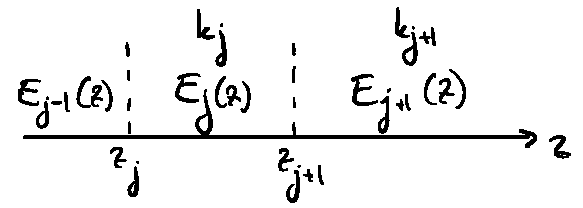
\includegraphics{Figures/SpaceDiscretion.pdf}
    }
\caption{
Caption
}
\label{fig:1}
\end{center}
\end{figure}

The interface between layer $j-1$ and $j$ is define as $\boldsymbol{\mathsf{r}}_j$. 
\begin{align*}
	\boldsymbol{\mathsf{r}}_j = x\vu{x} + y\vu{y} + z_j\vu{z}
\end{align*}
The electric field component at the interface need to respect the following equation
\begin{align*}
	\pqty{\vb{E}_{j-1}\pqty{\boldsymbol{\mathsf{r}}_j,t}}_{x,y} &= \pqty{\vb{E}_{j}\pqty{\boldsymbol{\mathsf{r}}_j,t}}_{x,y} \\
	\epsilon_{j-1}\pqty{\vb{E}_{j-1}\pqty{\boldsymbol{\mathsf{r}}_j,t}}_z &= \epsilon_{j}\pqty{\vb{E}_{j}\pqty{\boldsymbol{\mathsf{r}}_j,t}}_z
\end{align*} while the magnetic field components,
\begin{align*}
	\frac{1}{\mu_{j-1}}\pqty{\vb{B}_{j-1}\pqty{\boldsymbol{\mathsf{r}}_j,t}}_{x,y} &= \frac{1}{\mu_j}\pqty{\vb{B}_{j}\pqty{\boldsymbol{\mathsf{r}}_j,t}}_{x,y} \\
	\pqty{\vb{B}_{j-1}\pqty{\boldsymbol{\mathsf{r}}_j,t}}_z &= \pqty{\vb{B}_{j}\pqty{\boldsymbol{\mathsf{r}}_j,t}}_z 
\end{align*}

All these equation will have phase factors that must connect at the interface. 
\begin{align*}
	e^{i\pqty{\vb{k}_j^{(I,R)}\cdot\boldsymbol{\mathsf{r}}_j - \omega t}} = e^{-i\omega t}\exp i\pqty{k^{(I,R)}_{x,j}x + k^{(I,R)}_{y,j}y + k^{(I,R)}_{z,j}z_j}
\end{align*}

The $x$ and $y$ dependance must be the same on each side of each equation, meaning that, in each layer we must have
\begin{align*}
	k_{x,j} &= k^{(I)}_{x,j} = k^{(R)}_{x,j} & k_{y,j} &= k^{(I)}_{y,j} = k^{(R)}_{y,j} & k_{z,j} &= k^{(I)}_{z,j} = -k^{(R)}_{z,j}
\end{align*} and between planes
\begin{align*}
	k_{x,j-1} &= k_{x,j} & k_{y,j-1} &= k_{y,j}
\end{align*}

If we define $\theta_j$ as the angle between the interface and $\vb{k}_j$, we get the following relations (Snell's law).
\begin{align*}
	k_{j-1}\cos\theta_{j-1} &= k_{j}\cos\theta_{j} & \frac{\cos\theta_j}{\cos\theta_{j-1}} &= \frac{k_{j-1}}{k_j} = \frac{n_{j-1}}{n_j} = \pqty{\frac{\epsilon_{j-1}\mu_{j-1}}{\epsilon_j\mu_j}}^{1/2}
\end{align*}

If the first incident beam is $k_0$ at an angle $\theta_0$, this means,
\begin{align*}
	k_{0}\cos\theta_{0} &= k_{j}\cos\theta_{j} & \frac{k_0}{n_0} &= \frac{k_j}{n_j}
\end{align*}



% \begin{align*}
% 	\epsilon_{j-1}\pqty{E^{(I)}_{0z,j-1}e^{ik^{(I)}_{z,j-1}z_j} + E^{(R)}_{0z,j-1}e^{ik^{(R)}_{z,j-1}z_j}} &= 
% 	\epsilon_{j}\pqty{E^{(I)}_{0z,j}e^{ik^{(I)}_{z,j}z_j} + E^{(R)}_{0z,j}e^{ik^{(R)}_{z,j}z_j}} \\
% 	E^{(I)}_{0x,y,j-1}e^{ik^{(I)}_{z,j-1}z_j} + E^{(R)}_{0x,y,j-1}e^{ik^{(R)}_{z,j-1}z_j} &= 
% 	E^{(I)}_{0x,y,j}e^{ik^{(I)}_{z,j}z_j} + E^{(R)}_{0x,y,j}e^{ik^{(R)}_{z,j}z_j}
% \end{align*}

Polarisation in plane, with $k_y = 0$,
\begin{align*}
	E^{(I)}_{0x,j} &= E^{(I)}_{0,j}\sin\theta_j & E^{(R)}_{0x,j} &= -E^{(R)}_{0,j}\sin\theta_j \\
	E^{(I)}_{0y,j} &= 0 & E^{(R)}_{0y,j} &= 0 \\
	E^{(I)}_{0z,j} &= E^{(I)}_{0,j}\cos\theta_j & E^{(R)}_{0z,j} &= E^{(R)}_{0,j}\cos\theta_j
\end{align*}

\begin{align*}
	B^{(I)}_{0x,j} &= 0 & B^{(R)}_{0x,j} &= 0 \\
	\omega B^{(I)}_{0y,j} &= k^{(I)}_jE^{(I)}_{0,j} & \omega B^{(R)}_{0y,j} &= k^{(R)}_jE^{(R)}_{0,j} \\
	B^{(I)}_{0z,j} &= 0 & B^{(R)}_{0z,j} &= 0 \\
\end{align*}

The relevant equations are
\begin{align*}
	\sin\theta_{j-1}\pqty{E^{(I)}_{0,j-1}e^{ik_{z,j-1}z_j} + E^{(R)}_{0,j-1}e^{-ik_{z,j-1}z_j}} &=
	\sin\theta_{j}\pqty{E^{(I)}_{0,j}e^{ik_{z,j}z_j} - E^{(R)}_{0,j}e^{-ik_{z,j}z_j}} 
	\\
	\epsilon_{j-1} \cos\theta_{j-1} \pqty{E^{(I)}_{0,j-1}e^{ik_{z,j-1}z_j} + E^{(R)}_{0,j-1}e^{-ik_{z,j-1}z_j}} &=
	\epsilon_{j} \cos\theta_{j} \pqty{E^{(I)}_{0,j}e^{ik_{z,j}z_j} + E^{(R)}_{0,j} e^{-ik_{z,j}z_j}} 
	\\
	\frac{k_{j-1}}{\mu_{j-1}}\pqty{E^{(I)}_{0,j-1} e^{ik_{z,j-1}z_j} + E^{(R)}_{0,j-1} e^{ik_{z,j-1}z_j}} &=
	\frac{k_{j}}{\mu_{j}}\pqty{E^{(I)}_{0,j} e^{ik_{z,j}z_j} + E^{(R)}_{0,j} e^{ik_{z,j}z_j}}
\end{align*}

The third one is equivalent to the second one.

\begin{align*}
	\vb{W}_j \equiv \vb{S}_j\pqty{z}\cdot\vb{E}_j
\end{align*} where
\begin{align*}
	\vb{W}_j\pqty{\vb{r}} &= \pmqty{E_{0x,j}\pqty{\vb{r}} \\ \epsilon_j E_{0z,j}\pqty{\vb{r}}} = E_{0,j}\pqty{\vb{r}}\pmqty{\sin\theta_j \\ \epsilon_j \cos\theta_j}
	&\vb{E}_j &= \pmqty{E_{0,j}^{(I)} \\ E_{0,j}^{(R)}} 
	& 
	\vb{S}_j\pqty{z} &= \pmqty{
		\alpha_j e^{ik_{z,j}z} & 
		-\alpha_j e^{-ik_{z,j}z} \\
		\beta_j e^{ik_{z,j}z} & 
		\beta_j e^{-ik_{z,j}z}}
\end{align*} where we defined
% \begin{align*}
% 	\epsilon_j\cos\theta_j = \frac{n_j^2}{\mu_j}\cos\theta_j = \frac{\lambda n_j k_j}{\mu_j}\cos\theta_j
% \end{align*}
% \begin{align*}
% 	\frac{n_{j-1}}{\mu_{j-1}} \pqty{E^{(I)}_{0,j-1}e^{ik_{z,j-1}z_j} + E^{(R)}_{0,j-1}e^{-ik_{z,j-1}z_j}} &=
% 	\frac{n_{j}}{\mu_{j}} \pqty{E^{(I)}_{0,j}e^{ik_{z,j}z_j} + E^{(R)}_{0,j} e^{-ik_{z,j}z_j}} \\
% 	\pqty{1 - \frac{n_0^2\cos^2\theta_0}{n_{j-1}^2}}^{1/2}\pqty{E^{(I)}_{0,j-1}e^{ik_{z,j-1}z_j} + E^{(R)}_{0,j-1}e^{-ik_{z,j-1}z_j}} &=
% 	\pqty{1 - \frac{n_0^2\cos^2\theta_0}{n_{j}^2}}^{1/2}\pqty{E^{(I)}_{0,j}e^{ik_{z,j}z_j} + E^{(R)}_{0,j}e^{-ik_{z,j}z_j}}
% \end{align*}
% \begin{align*}
% 	E^{(I)}_{0,j-1}e^{ik_{z,j-1}z_j} + E^{(R)}_{0,j-1}e^{-ik_{z,j-1}z_j} &=
% 	\frac{\epsilon_j}{\epsilon_{j-1}}\frac{\cos\theta_j}{\cos\theta_{j-1}} \pqty{E^{(I)}_{0,j}e^{ik_{z,j}z_j} + E^{(R)}_{0,j} e^{-ik_{z,j}z_j}}  
% 	% \\
% 	% E^{(I)}_{0,j-1} e^{ik_{z,j-1}z_j} + E^{(R)}_{0,j-1} e^{ik_{z,j-1}z_j} &=
% 	% \frac{k_{j}}{k_{j-1}}\frac{\mu_{j-1}}{\mu_{j}}\pqty{E^{(I)}_{0,j} e^{ik_{z,j}z_j} + E^{(R)}_{0,j} e^{ik_{z,j}z_j}}
% \end{align*}
\begin{align*}
	\alpha_j &\equiv \sin\theta_j = \pqty{1 - \frac{n_0^2\cos^2\theta_0}{n_{j}^2}}^{1/2} & \beta_j &\equiv \epsilon_j\cos\theta_j  = \frac{n_j}{\mu_j} \lambda k_0 \cos\theta_0
\end{align*}so that,
\begin{align*}
	\vb{W}_{j-1}\pqty{\boldsymbol{\mathsf{r}}_j,t} &= \vb{W}_{j}\pqty{\boldsymbol{\mathsf{r}}_j,t}
\end{align*}

\begin{align*}
	\det{\vb{S}_j} &= 2\alpha_j\beta_j = 2\epsilon_j\sin\theta_j\cos\theta_j = 2n^2_j\sin\theta_j\cos\theta_j = 2n_j\sin\theta_j n_0\cos\theta_0
\end{align*}

Polarisation out of plane, with $k_y = 0$,
\begin{align*}
	E^{(I)}_{0x,j} &= 0 & E^{(R)}_{0x,j} &= 0 \\
	E^{(I)}_{0y,j} &= E^{(I)}_{0,j} & E^{(R)}_{0y,j} &= E^{(R)}_{0,j} \\
	E^{(I)}_{0z,j} &= 0 & E^{(R)}_{0z,j} &= 0 \\
\end{align*}

\begin{align*}
	\omega B^{(I)}_{0x,j} &= k_j E^{(I)}_{0,j}\sin\theta_j & \omega B^{(R)}_{0x,j} &= -k_j E^{(R)}_{0,j}\sin\theta_j \\
	B^{(I)}_{0y,j} &= 0 & B^{(R)}_{0y,j} &= 0 \\
	\omega B^{(I)}_{0z,j} &= k_j E^{(I)}_{0,j}\cos\theta_j & \omega B^{(R)}_{0z,j} &= k_j E^{(R)}_{0,j}\cos\theta_j \\
\end{align*}

The relevant equations are
\begin{align*}
	E^{(I)}_{0,j-1}e^{ik_{z,j-1}z_j} + E^{(R)}_{0,j-1}e^{-ik_{z,j-1}z_j} &=
	E^{(I)}_{0,j}e^{ik_{z,j}z_j} + E^{(R)}_{0,j} e^{-ik_{z,j}z_j}
	\\
	k_{j-1}\sin\theta_{j-1}\pqty{E^{(I)}_{0,j-1}e^{ik_{z,j-1}z_j} + E^{(R)}_{0,j-1}e^{-ik_{z,j-1}z_j}} &=
	k_{j}\sin\theta_{j}\pqty{E^{(I)}_{0,j}e^{ik_{z,j}z_j} - E^{(R)}_{0,j}e^{-ik_{z,j}z_j}} 
	% \\
	% k_{j-1}\cos\theta_{j-1}\pqty{E^{(I)}_{0,j-1}e^{ik_{z,j-1}z_j} + E^{(R)}_{0,j-1}e^{-ik_{z,j-1}z_j}} &=
	% k_{j-1}\cos\theta_{j}\pqty{E^{(I)}_{0,j}e^{ik_{z,j}z_j} + E^{(R)}_{0,j}e^{-ik_{z,j}z_j}} 
\end{align*}

\begin{align*}
	\vb{W}_j\pqty{\vb{r}} &= \pmqty{E_{0y,j}\pqty{\vb{r}} \\ \omega B_{0x,j}\pqty{\vb{r}} } = E_{0,j}\pqty{\vb{r}}\pmqty{1 \\ k_j\sin\theta_j  } 
	&\vb{E}_j &= \pmqty{E_{0,j}^{(I)} \\ E_{0,j}^{(R)}} 
	& 
	\vb{S}_j\pqty{z} &= \pmqty{
		e^{ik_{z,j}z} & 
		e^{-ik_{z,j}z}  \\
		k_{z,j} e^{ik_{z,j}z} & 
		-k_{z,j} e^{-ik_{z,j}z}
		}
\end{align*} with
\begin{align*}
	k_{z,j} &\equiv k_{j}\sin\theta_{j} = k_j\alpha_j = \frac{2\pi n_j\alpha_j}{\lambda}
\end{align*}

For X-Rays both polarisation can pe approximate by the later one.

Lets note that $\det{\vb{S}_j} = -2k_{z,j}$.

In both polarisation what we have at the interface is,
\begin{align*}
	\vb{W}_{j-1}\pqty{\boldsymbol{\mathsf{r}}_j,t} &= \vb{W}_{j}\pqty{\boldsymbol{\mathsf{r}}_j,t}
\end{align*}

In case of $n_j < \cos\theta_j$, $k_{z,j}$ is imaginary. We define $\kappa_z = \mathcal{I}\qty{k_z}$ and,
\begin{align*}
	\vb{S}_j\pqty{z} &= \pmqty{
		e^{ik_{z,j}z} & 
		e^{-ik_{z,j}z}  \\
		k_{z,j} e^{ik_{z,j}z} & 
		-k_{z,j} e^{-ik_{z,j}z}
		} &
	\vb{S}_j\pqty{z} &= \pmqty{
		e^{-\kappa_{z,j}z} & 
		e^{\kappa_{z,j}z}  \\
		i\kappa_{z,j} e^{-\kappa_{z,j}z} & 
		-i\kappa_{z,j} e^{\kappa_{z,j}z}
		}
\end{align*}

\begin{align*}
	k_{z,j} \to i\kappa_{z,j}
\end{align*}

\subsection{Interface transfer} % (fold)
\label{sub:interface_transfer}

% subsection interface_transfer (end)

We define the transfer matrix as,
\begin{align*}
	\vb{E}_j = \vb{T}_j \cdot \vb{E}_{j-1}
\end{align*}

We can find this matrix with the help of the interface condition,
\begin{align*}
	\vb{W}_j\pqty{\boldsymbol{\mathsf{r}}_j} &= \vb{W}_{j-1}\pqty{\boldsymbol{\mathsf{r}}_j} \\
	\vb{S}_j\pqty{\boldsymbol{\mathsf{r}}_j} \cdot \vb{E}_j &= \vb{S}_{j-1}\pqty{\boldsymbol{\mathsf{r}}_j} \cdot \vb{E}_{j-1}
\end{align*} so that,
\begin{align*}
	\vb{T}_j = \vb{S}^{-1}_j\pqty{\boldsymbol{\mathsf{r}}_j} \cdot\vb{S}_{j-1}\pqty{\boldsymbol{\mathsf{r}}_j}
\end{align*}

Let's note that $\det{\vb{T}_j} = \frac{k_{j-1}}{k_{j}}$.
\begin{align*}
	\vb{T}_j &=
	\frac{1}{2k_{z,j}}\pmqty{
		k_{z,j} e^{-ik_{z,j}z_j} & 
		e^{-ik_{z,j}z_j}  \\
		k_{z,j} e^{ik_{z,j}z_j} & 
		-e^{ik_{z,j}z_j}
		} \pmqty{
	e^{ik_{z,j-1}z_j} & 
	e^{-ik_{z,j-1}z_j}  \\
	k_{z,j-1} e^{ik_{z,j-1}z_j} & 
	-k_{z,j-1} e^{-ik_{z,j-1}z_j}
	}  \\
	% &= \frac{1}{2k_{z,j}}\pmqty{
	% 	k_{z,j} e^{-ik_{z,j}z_j}e^{ik_{z,j-1}z_j} 
	% 		+ e^{-ik_{z,j}z_j}k_{z,j-1} e^{ik_{z,j-1}z_j} &
	% 	k_{z,j} e^{-ik_{z,j}z_j}e^{-ik_{z,j-1}z_j} 
	% 	    - e^{-ik_{z,j}z_j}k_{z,j-1} e^{-ik_{z,j-1}z_j}  \\
	% 	k_{z,j} e^{ik_{z,j}z_j}e^{ik_{z,j-1}z_j} 
	% 	    - e^{ik_{z,j}z_j}k_{z,j-1} e^{ik_{z,j-1}z_j} &
	% 	k_{z,j} e^{ik_{z,j}z_j}e^{-ik_{z,j-1}z_j} 
	% 	    + e^{ik_{z,j}z_j}k_{z,j-1} e^{-ik_{z,j-1}z_j}
	% 	} \\
	% &= \frac{1}{2k_{z,j}}\pmqty{
	% 	\pqty{k_{z,j} + k_{z,j-1}}e^{-ik_{z,j}z_j}e^{ik_{z,j-1}z_j} &
	% 	\pqty{k_{z,j} - k_{z,j-1}}e^{-ik_{z,j}z_j}e^{-ik_{z,j-1}z_j}  \\
	% 	\pqty{k_{z,j} - k_{z,j-1}}e^{ik_{z,j}z_j}e^{ik_{z,j-1}z_j} &
	% 	\pqty{k_{z,j} + k_{z,j-1}}e^{ik_{z,j}z_j}e^{-ik_{z,j-1}z_j}
	% 	} \\
	&= \frac{1}{2k_{z,j}}\pmqty{
		\pqty{k_{z,j} + k_{z,j-1}}e^{-i\pqty{k_{z,j} - k_{z,j-1}}z_j} &
		\pqty{k_{z,j} - k_{z,j-1}}e^{-i\pqty{k_{z,j} + k_{z,j-1}}z_j}  \\
		\pqty{k_{z,j} - k_{z,j-1}}e^{ i\pqty{k_{z,j} + k_{z,j-1}}z_j} &
		\pqty{k_{z,j} + k_{z,j-1}}e^{ i\pqty{k_{z,j} - k_{z,j-1}}z_j}
		} \\
\end{align*}

\begin{align*}
	\vb{T}_j &=
		\frac{1}{2\kappa_{z,j}}\pmqty{
		\pqty{\kappa_{z,j} + \kappa_{z,j-1}}e^{\pqty{\kappa_{z,j} - \kappa_{z,j-1}}z_j} &
		\pqty{\kappa_{z,j} - \kappa_{z,j-1}}e^{\pqty{\kappa_{z,j} + \kappa_{z,j-1}}z_j}  \\
		\pqty{\kappa_{z,j} - \kappa_{z,j-1}}e^{ -\pqty{\kappa_{z,j} + \kappa_{z,j-1}}z_j} &
		\pqty{\kappa_{z,j} + \kappa_{z,j-1}}e^{ -\pqty{\kappa_{z,j} - \kappa_{z,j-1}}z_j}
		} \\
\end{align*}


% \begin{align*}
% 	\vb{T}_j &\approx \pmqty{
% 		e^{-i\pqty{k_{z,j} - k_{z,j-1}}z_j} &
% 		\frac{k_{z,j} - k_{z,j-1}}{k_{z,j} + k_{z,j-1}}e^{-i\pqty{k_{z,j} + k_{z,j-1}}z_j}  \\
% 		\frac{k_{z,j} - k_{z,j-1}}{k_{z,j} + k_{z,j-1}}e^{ i\pqty{k_{z,j} + k_{z,j-1}}z_j} &
% 		e^{ i\pqty{k_{z,j} - k_{z,j-1}}z_j}
% 		} \\
% \end{align*}

To go from the first interface to the last we just need to apply the matrices in sequence.
\begin{align*}
	\vb{E}_N &= \vb{L}\cdot\vb{E}_0 & \vb{L} &= \vb{T}_N\cdot\vb{T}_{N-1}\cdots\vb{T}_2\cdot\vb{T}_{1} = \prod_{n=1}^N \vb{T}_n 
\end{align*}

\begin{align*}
	\pmqty{t\\ 0} &= \pmqty{L_{11} & L_{12}\\L_{21}&L_{22}}\cdot\pmqty{1\\r}
\end{align*}

\begin{align*}
	r &= -\frac{L_{21}}{L_{22}} & t = L_{11} - \frac{L_{12}L_{21}}{L_{22}}  = \frac{\det{\vb{L}}}{L_{22}}
\end{align*}

Let's note that $\det{\vb{L}} = \prod_{j=1}^N\frac{k_{j-1}}{k_{j}} = \frac{k_0}{k_N}$ if $k_j > 0$ and $0$ otherwise.

% If X-rays can't penetrate layer $J+1$ the relevant equation become,
% \begin{align*}
% 	E^{(I)}_{0,J}e^{ik_{z,J}z_{J+1}} + E^{(R)}_{0,J}e^{-ik_{z,J}z_{J+1}} &=
% 	0
% \end{align*}

% \begin{align*}
% 	E^{(R)}_{0,J} = -E^{(I)}_{0,J}e^{i2k_{z,J}z_{J+1}}
% \end{align*}

% \begin{align*}
% 	\vb{E}_{J} = E^{(I)}_{0,J}\pmqty{1 \\-e^{i2k_{z,J}z_{J+1}}}
% \end{align*}

% \begin{align*}
% 	\vb{E}_J &= \vb{L}\cdot\vb{E}_0 & \vb{L} &= \vb{T}_J\cdot\vb{T}_{J-1}\cdots\vb{T}_2\cdot\vb{T}_{1} = \prod_{n=1}^J \vb{T}_n 
% \end{align*}

% \begin{align*}
% 	E^{(I)}_{0,J}\pmqty{1\\ -e^{i2k_{z,J}z_{J+1}}} &= A\pmqty{L_{11} & L_{12}\\L_{21}&L_{22}}\cdot\pmqty{1\\r}
% \end{align*}

% \begin{align*}
% 	C &= L_{11} + L_{12}r \\
% 	-e^{i2k_{z,J}z_{J+1}} C &= L_{21} + L_{22}r
% \end{align*}

% \begin{align*}
% 	 r &= -\frac{L_{21} + e^{i2k_{z,J}z_{J+1}}L_{11}}{L_{22} + e^{i2k_{z,J}z_{J+1}} L_{12}}
% \end{align*}

\subsection{Roughness} % (fold)
\label{sub:roughness}

\begin{align*}
	\vb{L} &= \int\dd{z} p_j\pqty{z}\vb{T}_N\cdots\vb{T}_j\pqty{z}\cdots\cdot\vb{T}_{1} \\
	&= \vb{T}_N\cdots\pqty{\int\dd{z} p_j\pqty{z}\vb{T}_j\pqty{z}}\cdots\cdot\vb{T}_{1}
\end{align*}

\begin{align*}
	p_j\pqty{z} = \frac{1}{\sigma_j\sqrt{2\pi}}\exp{-\frac{1}{2}\pqty{\frac{z - z_j}{\sigma_j}}^2}
\end{align*}

\begin{align*}
	\int\dd{z}p_j\pqty{z}e^{i\pqty{k_{z,j} \pm k_{z,j-1}}z} &= 
	e^{i\pqty{k_{z,j} \pm k_{z,j-1}}z_j} 
	e^{-\frac{1}{2}\pqty{k_{z,j} \pm k_{z,j-1}}^2\sigma_j^2}
\end{align*}

\begin{align*}
	\int\dd{z}p_j\pqty{z} \vb{T}_j\pqty{z} \\= \frac{1}{2k_{z,j}}\pmqty{
		\pqty{k_{z,j} + k_{z,j-1}}e^{-i\pqty{k_{z,j} - k_{z,j-1}}z_j}
			e^{-\frac{1}{2}\pqty{k_{z,j} - k_{z,j-1}}^2\sigma_j^2} &
		\pqty{k_{z,j} - k_{z,j-1}}e^{-i\pqty{k_{z,j} + k_{z,j-1}}z_j}
			e^{-\frac{1}{2}\pqty{k_{z,j} + k_{z,j-1}}^2\sigma_j^2}  \\
		\pqty{k_{z,j} - k_{z,j-1}}e^{ i\pqty{k_{z,j} + k_{z,j-1}}z_j}
			e^{-\frac{1}{2}\pqty{k_{z,j} + k_{z,j-1}}^2\sigma_j^2} &
		\pqty{k_{z,j} + k_{z,j-1}}e^{ i\pqty{k_{z,j} - k_{z,j-1}}z_j}
			e^{-\frac{1}{2}\pqty{k_{z,j} - k_{z,j-1}}^2\sigma_j^2}
		}
\end{align*}

\begin{align*}
	\int\dd{z}p_j\pqty{z} \vb{T}_j\pqty{z} &\approx \frac{1}{2k_{z,j}}\pmqty{
		2k_{z,j}e^{-i\pqty{k_{z,j} - k_{z,j-1}}z_j} &
		\pqty{k_{z,j} - k_{z,j-1}}e^{-i\pqty{k_{z,j} + k_{z,j-1}}z_j}
			e^{-\frac{1}{2}\pqty{k_{z,j} + k_{z,j-1}}^2\sigma_j^2}  \\
		\pqty{k_{z,j} - k_{z,j-1}}e^{ i\pqty{k_{z,j} + k_{z,j-1}}z_j}
			e^{-\frac{1}{2}\pqty{k_{z,j} + k_{z,j-1}}^2\sigma_j^2} &
		\pqty{k_{z,j} + k_{z,j-1}}e^{ i\pqty{k_{z,j} - k_{z,j-1}}z_j}
			e^{-\frac{1}{2}\pqty{k_{z,j} - k_{z,j-1}}^2\sigma_j^2}
		}
\end{align*}

\subsection{Layer Transfer} % (fold)
\label{sub:layer_transfer}

We define the transfer matrix as,
\begin{align*}
	\vb{W}_j\pqty{z_{j+1}} = \vb{M}_j \cdot \vb{W}_j\pqty{z_{j}}
\end{align*}

We can find this matrix with the help $\vb{E}$
\begin{align*}
	\vb{S}_j\pqty{z_{j+1}}\cdot \vb{E}_j = \vb{M}_j \cdot \vb{S}_j\pqty{z_{j}}\cdot \vb{E}_j
\end{align*}

So that,
\begin{align*}
	\vb{M}_j &= \vb{S}_j\pqty{z_{j+1}} \cdot \vb{S}^{-1}_j\pqty{z_{j}}
\end{align*}

\begin{align*}
	\vb{M}_j 
	&=
	\pmqty{
		e^{ik_{z,j}z_{j+1}} & 
		e^{-ik_{z,j}z_{j+1}}  \\
		k_{z,j} e^{ik_{z,j}z_{j+1}} & 
		-k_{z,j} e^{-ik_{z,j}z_{j+1}}
	} \frac{1}{2k_{z,j}}\pmqty{
		k_{z,j} e^{-ik_{z,j}z_j} & 
		e^{-ik_{z,j}z_j}  \\
		k_{z,j} e^{ik_{z,j}z_j} & 
		-e^{ik_{z,j}z_j}
		} \\
	% &= \frac{1}{2k_{z,j}}\pmqty{
	% 	e^{ik_{z,j}z_{j+1}}k_{z,j} e^{-ik_{z,j}z_j} + e^{-ik_{z,j}z_{j+1}}k_{z,j} e^{ik_{z,j}z_j} &
	% 	e^{ik_{z,j}z_{j+1}}e^{-ik_{z,j}z_j} - e^{-ik_{z,j}z_{j+1}}e^{ik_{z,j}z_j} \\
	% 	k_{z,j} e^{ik_{z,j}z_{j+1}}k_{z,j} e^{-ik_{z,j}z_j} - k_{z,j} e^{-ik_{z,j}z_{j+1}}k_{z,j} e^{ik_{z,j}z_j} &
	% 	k_{z,j} e^{ik_{z,j}z_{j+1}}e^{-ik_{z,j}z_j} + k_{z,j} e^{-ik_{z,j}z_{j+1}}e^{ik_{z,j}z_j}
	% } \\
	&= \frac{1}{2k_{z,j}} 
	\pmqty{
		\cos\pqty{k_{z,j}d_j} &
		i k_{z,j}^{-1}\sin\pqty{k_{z,j}d_j} \\
		i k_{z,j} \sin\pqty{k_{z,j}d_j} &
		\cos\pqty{k_{z,j}d_j}
	}
\end{align*}

To go from the first interface to the last we just need to apply the matrices in sequence.
\begin{align*}
	\vb{L} &= \vb{S}_N\pqty{z_N}^{-1}\cdot\vb{M}_{N-1}\cdot\vb{M}_{N-2} \cdots \vb{M}_{2}\cdot\vb{M}_{1}\cdot \vb{S}_0\pqty{z_1}
\end{align*}

\begin{align*}
	r = -e^{i2k_z\pqty{a}a}\frac{
		k_z\pqty{b} - k_z\pqty{a} + \pqty{b-a} k_z\pqty{a} k_z\pqty{b}  - \int_a^b \dd{z} k_{z}^2\pqty{z}  
		}{
		k_z\pqty{b} + k_z\pqty{a} - \pqty{b-a}k_z\pqty{a} k_z\pqty{b}  - \int_a^b \dd{z} k_{z}^2\pqty{z}  
		}
\end{align*}


% subsection layer_transfer (end)

% subsection roughness (end)
%!TEX root = ../Theory.tex

\section{Geometry} % (fold)
\label{sec:geometry}

% section geometry (end)

\subsection{Vecteurs de base réseau direct}

\begin{align*}
	\vb{a}_1 && \vb{a}_2 && \vb{a}_3
\end{align*} 

\subsection{Vecteurs de base réseau réciproque}

On construit les vecteur de base du réseau réciproque de manière à ce que les $\vb{b}_i$ soient orthogonaux aux $\vb{a}_j$ pour $i \neq j$. 
\begin{align*}
	\vb{b}_i = \frac{\pi}{V} \epsilon_{ijk} \vb{a}_j \times \vb{a}_k
\end{align*} où on divise par deux car on compte $\vb{a}_j \times \vb{a}_k - \vb{a}_k \times \vb{a}_j$. 

\subsection{Produit scalaire espace direct}
\label{ssec:dotRR}

Le produits sclaire entre deux vecteurs de base du réseau cristalin implique les longueurs et l'angle mutuelle,
\begin{align*}
	\vb{a}_i\cdot\vb{a}_j = a_i a_j \cos\alpha_{ij}.
\end{align*}

\subsection{Produit scalaire espace reciproque}
Le produit scalaire de deux vecteurs de la base du réseau réciproque peut être exprimé à l'aide de produits des vecteurs de base du réseau direct,
\begin{align*}
	\vb{b}_i \cdot \vb{b}_j 
	% &= \pqty{\frac{\pi}{V}}^2 \pqty{\epsilon_{imn} \vb{a}_m \times \vb{a}_n} \cdot \pqty{\epsilon_{jpq} \vb{a}_p \times \vb{a}_q} \\
	&= \pqty{\frac{\pi}{V}}^2 \epsilon_{imn} \epsilon_{jpq} \pqty{ \vb{a}_m \times \vb{a}_n}\cdot\pqty{ \vb{a}_p \times \vb{a}_q}.
\end{align*}

On utilise l'identité vectorielle suivante,
\begin{align*}
	\pqty{ \vb{a}_m \times \vb{a}_n}\cdot\pqty{ \vb{a}_p \times \vb{a}_q} = \pqty{\vb{a}_m\cdot\vb{a}_p}\pqty{\vb{a}_n\cdot\vb{a}_q} - \pqty{\vb{a}_m\cdot\vb{a}_q}\pqty{\vb{a}_n\cdot\vb{a}_p}
\end{align*} pour exprimé le résultat en fonction de produit scalaire uniquement,
\begin{align*}
	\vb{b}_i \cdot \vb{b}_j 
	&= \pqty{\frac{\pi}{V}}^2 \epsilon_{imn} \epsilon_{jpq} \bqty{\pqty{\vb{a}_m\cdot\vb{a}_p}\pqty{\vb{a}_n\cdot\vb{a}_q} - \pqty{\vb{a}_m\cdot\vb{a}_q}\pqty{\vb{a}_n\cdot\vb{a}_p}}.
\end{align*}

À l'aide de \ref{ssec:dotRR}, on obtient donc,
\begin{align*}
	\vb{b}_i \cdot \vb{b}_j 
	&= \pqty{\frac{\pi}{V}}^2 \epsilon_{imn} \epsilon_{jpq} a_m a_n a_p a_q \bqty{\cos\alpha_{mp}\cos\alpha_{nq} - \cos\alpha_{mq}\cos\alpha_{np}}.
\end{align*}

\subsection{Produit scalaire croisé}
Par construction le produit scalaire entre un vecteur de la base directe et un vecteur de la base réciproque est,
\begin{align*}
	\vb{a}_i \cdot \vb{b}_j = 2\pi \delta_{ij}
\end{align*}

\subsection{Produit vectoriel espace direct}
La définion des vecteurs de base du réseau réciproque contient le produit vectoriel des vecteurs de base du réseaud direct. Pour extraire, le résultat du produit on multiplie simplement par le tenseur de Levi-Civita,
\begin{align*}
	\vb{b}_i\epsilon_{imn} &= \frac{\pi}{V}\epsilon_{imn} \epsilon_{ijk} \vb{a}_j \times \vb{a}_k \\
	&= \frac{\pi}{V}\pqty{\delta_{mj}\delta_{nk} - \delta_{mk}\delta_{nj}} \vb{a}_j \times \vb{a}_k \\
	&= \frac{\pi}{V}\pqty{\vb{a}_m \times \vb{a}_n - \vb{a}_n \times \vb{a}_m} \\
	&= \frac{2\pi}{V}\vb{a}_m \times \vb{a}_n
\end{align*}

On peut alors isoler le résultat,
\begin{align*}
	\vb{a}_m \times \vb{a}_n &=\frac{V}{2\pi} \epsilon_{imn} \vb{b}_i
\end{align*}


\subsection{Produit vectoriel espace réciproque}
Le produit vectorielle entre les vecteurs de base du réseau réciproque prend la forme d'un produit quadruple
\begin{align*}
	\vb{b}_i \times \vb{b}_l &= \pqty{\frac{\pi}{V}}^2 \epsilon_{ijk} \epsilon_{lmn} \pqty{\vb{a}_j \times \vb{a}_k} \times \pqty{\vb{a}_m \times \vb{a}_n}
\end{align*} qui peut être réexprimé sous la forme du produit triple.
\begin{align*}
	\pqty{\vb{a}_j \times \vb{a}_k} \times \pqty{\vb{a}_m \times \vb{a}_n} &= 
	\bqty{\vb{a}_j,\vb{a}_k,\vb{a}_n} \vb{a}_m - \bqty{\vb{a}_j,\vb{a}_k,\vb{a}_m} \vb{a}_n
\end{align*}

Le produit triple des vecteurs de base du réseau cristallin donne le volume de la maille élémentaire. Ce produit peut être fait dans les deux sens.
\begin{align*}
	\bqty{\vb{a}_j,\vb{a}_k,\vb{a}_n} = V \epsilon_{jkn} - V\epsilon_{nkj}
\end{align*}

Cela nous permet d'écrire le produit vectorielle de deux vecteur de base du réseau réciproque comme une combinaison linéaire des vecteur de base du réseau cristlin.
\begin{align*}
	\vb{b}_i \times \vb{b}_l &= \frac{\pqty{2\pi}^2}{V} \epsilon_{ilm} \vb{a}_m
\end{align*}

\subsection{Produit vectoriel croisé}
\begin{align*}
	\vb{a}_i \times \vb{b}_j &= \frac{\pi}{V}\epsilon_{jmn}\vb{a}_i \times\pqty{\vb{a}_m \times \vb{a}_n} \\
	&= \frac{\pi}{V}\epsilon_{jmn} \bqty{\pqty{\vb{a}_i \cdot \vb{a}_n}\vb{a}_m - \pqty{\vb{a}_i \cdot \vb{a}_m}\vb{a}_n} \\
	&= \frac{2\pi}{V}\epsilon_{jmn} \pqty{\vb{a}_i \cdot \vb{a}_n}\vb{a}_m \\
	&= \frac{2\pi}{V}\epsilon_{jmn} a_ia_n\cos\alpha_{in}\vb{a}_m
\end{align*}

\subsection{Volume cellule unité}
Par définition le volume de la cellule unité est,
\begin{align*}
	V = \vb{a}_1 \cdot \pqty{\vb{a}_2 \times \vb{a}_3}
\end{align*}

Il est plus pratique d'exprimer le carré de ce volume,
\begin{align*}
	V^2 &= \pqty{\vb{a}_1 \cdot \pqty{\vb{a}_2 \times \vb{a}_3}}\pqty{\vb{a}_1 \cdot \pqty{\vb{a}_2 \times \vb{a}_3}} \\
		&= \det{\pmqty{
		\vb{a}_1 \cdot \vb{a}_1 & \vb{a}_1 \cdot \vb{a}_2 & \vb{a}_1 \cdot \vb{a}_3 \\
		\vb{a}_2 \cdot \vb{a}_1 & \vb{a}_2 \cdot \vb{a}_2 & \vb{a}_2 \cdot \vb{a}_3 \\
		\vb{a}_3 \cdot \vb{a}_1 & \vb{a}_3 \cdot \vb{a}_2 & \vb{a}_3 \cdot \vb{a}_3
	}} \\
		&= \det{\pmqty{
		a_1^2 & a_1a_2\cos\alpha_{12} & a_1a_3\cos\alpha_{13} \\
		a_1a_2\cos\alpha_{12} & a_2^2 & a_2a_3\cos\alpha_{23} \\
		a_1a_3\cos\alpha_{13} & a_2a_3\cos\alpha_{23}  & a_3^2
	}} \\
	&= a_1^2 a_2^2 a_3^2 \pqty{1 + 2\cos\alpha_{12}\cos\alpha_{23}\cos\alpha_{13} - \cos^2\alpha_{12} - \cos^2\alpha_{23} - \cos^2\alpha_{13}}
\end{align*}

\subsection{Vecteur du réseau direct}

Les vecteurs du réseau direct peuvent être construits grâce au trio d'entier $pqr$ :
\begin{align*}
	\vb{R}_{pqr} = p \vb{a_1} + q \vb{a_2} + r \vb{a_3}.
\end{align*}

\subsection{Vecteur du réseau réciproque}

Les vecteurs du réseau réciproque peuvent être construits grâce au trio d'entier $hkl$ :
\begin{align*}
	\vb{G}_{hkl} = h \vb{b_1} + k \vb{b_2} + l \vb{b_3}.
\end{align*}



\subsection{Produit scalaire direct}
\begin{align*}
	\vb{R}_{pqr} \cdot \vb{R}_{p^\prime q^\prime r^\prime} = 
	pp^\prime \vb{a_1}\cdot\vb{a_1} + qq^\prime \vb{a_2}\cdot\vb{a_2} + rr^\prime \vb{a_3}\cdot\vb{a_3}
	+\pqty{pq^\prime + qp^\prime} \vb{a_1}\cdot\vb{a_2} + \pqty{qr^\prime + rq^\prime} \vb{a_2}\cdot\vb{a_3} + \pqty{rp^\prime + pr^\prime} \vb{a_3}\cdot\vb{a_1}.
\end{align*}

\subsection{Produit scalaire réciproque}
Le produit scalaire entre deux de ces vecteur s'exprime, en générale, de la manière suivante,
\begin{align*}
	\vb{G}_{hkl} \cdot \vb{G}_{h^\prime k^\prime l^\prime} = 
	hh^\prime \vb{b_1}\cdot\vb{b_1} + kk^\prime \vb{b_2}\cdot\vb{b_2} + ll^\prime \vb{b_3}\cdot\vb{b_3}
	+\pqty{hk^\prime + kh^\prime} \vb{b_1}\cdot\vb{b_2} + \pqty{kl^\prime + lk^\prime} \vb{b_2}\cdot\vb{b_3} + \pqty{lh^\prime + hl^\prime} \vb{b_3}\cdot\vb{b_1}.
\end{align*}

\subsection{Produit scalaire croisé}
\begin{align*}
	\vb{R}_{pqr} \cdot \vb{G}_{hkl} = ph + qk + rl
\end{align*}

\subsection{Produit vectoriel direct}

\begin{align*}
	\vb{R} \times \vb{R}^\prime &= p_i p_j^\prime \vb{a}_i \times \vb{a}_j \\
	&= \frac{V}{2\pi} \epsilon_{ijk} p_i p_j^\prime \vb{b}_k
\end{align*}

\subsection{Produit vectoriel réciproque}
\begin{align*}
	\vb{G} \times \vb{G}^\prime &= h_i h_j^\prime \vb{b}_i \times \vb{b}_j \\
	&= \frac{\pqty{2\pi}^2}{V} \epsilon_{ijk}  h_i h_j^\prime  \vb{a}_k
\end{align*}

\subsection{Produit vectoriel croisé}
\begin{align*}
	\vb{G} \times \vb{R} &= h_i p_j \vb{b}_i \times \vb{a}_j \\
	&= \frac{2\pi}{V} \epsilon_{jmn} h_i p_j  a_ia_n\cos\alpha_{in}\vb{a}_m \\
	&= \frac{2\pi}{V} \epsilon_{jmn} h_i p_j  \pqty{\vb{a}_i \cdot \vb{a}_n}\vb{a}_m
\end{align*}


\subsection{Angle entre deux vecteur du réseau réciproque} % (fold)
\label{sub:angle_entre_deux_vecteur_du_réseau_réciproque}

Grâce au produit sclaire, on peut être l'angle entre ces deux vecteurs.
\begin{align*}
	\cos\theta_{hkl,h^\prime k^\prime l^\prime} = \frac{\vb{G}_{hkl} \cdot \vb{G}_{h^\prime k^\prime l^\prime}}{\abs{\vb{G}_{hkl}}  \abs{\vb{G}_{h^\prime k^\prime l^\prime}}} = \frac{\vb{G}_{hkl} \cdot \vb{G}_{h^\prime k^\prime l^\prime}}{\pqty{\vb{G}_{hkl} \cdot \vb{G}_{hkl}}^{1/2}\pqty{\vb{G}_{h^\prime k^\prime l^\prime} \cdot \vb{G}_{h^\prime k^\prime l^\prime}}^{1/2}} 
\end{align*}


\subsection{Projection sur un vecteur du réseau réciproque} 

Projeté sur $\vb{G}_{HKL}$,
\begin{align*}
	\pqty{\vb{G}_{hkl}}_{\parallel\vb{G}_{HKL}} = \frac{\vb{G}_{HKL} \cdot \vb{G}_{hkl}}{\vb{G}_{HKL} \cdot \vb{G}_{HKL} }\vb{G}_{HKL} 
\end{align*}

Projeté sur le plan,
\begin{align*}
	\pqty{\vb{G}_{hkl}}_{\perp\vb{G}_{HKL}} = \vb{G}_{hkl} - \frac{\vb{G}_{HKL} \cdot \vb{G}_{hkl}}{\vb{G}_{HKL} \cdot \vb{G}_{HKL} }\vb{G}_{HKL} 
\end{align*}

\paragraph{Produit de phase} % (fold)
\label{par:produit_de_phase}

$\vb{G} \cdot \vb{r}$

\begin{align*}
	\vb{G} &= h_i \vb{b}_i & \vb{r} = \eta_j \vb{a}_j
\end{align*}

\begin{align*}
	\vb{G} \cdot \vb{r} 
	&= h_i \eta_j \vb{b}_i \cdot \vb{a}_j \\
	&= 2 \pi h_i \eta_j
\end{align*}

\section{Espace} % (fold)
\label{sec:espace}

On peut définir la position d'un réseau dans l'espace en stipulant la direction d'un vecteur du réseau réciproque selon $\vu{z}$ et un vecteur du réseau cristalin selon $\vu{x}$ :
\begin{align*}
	\vb{G}^{(z)} = G^{(z)}\vu{z} \qq{et} \vb{R}^{(x)} = R^{(x)} \vu{x}
\end{align*} où
\begin{align*}
	\vb{R}_{pqr} = p \vb{a_1} + q \vb{a_2} + r \vb{a_3}
\end{align*}

Ces deux vecteur doivent être orthogonaux et donc
\begin{align*}
	\vb{G}^{(z)} \cdot \vb{R}^{(x)} &= 2\pi\pqty{ h^{(z)}p^{(x)} + k^{(z)}q^{(x)} + l^{(z)}r^{(x)}} = G^{(z)}R^{(x)} \vu{z} \cdot \vu{x} = 0
\end{align*}

On peut obtenir les composantes selon $\vu{z}$ et $\vu{x}$ d'un vecteur du réseau réciproque dans cette espace en le projetant sur $\vb{G}^{(z)}$, $\vb{R}^{(x)}$. 
\begin{align*}
	\vb{G}_{hkl} \cdot \vu{z} &= \frac{\vb{G}_{hkl} \cdot \vb{G}^{(z)}}{\abs{\vb{G}^{(z)}}} &
	\vb{G}_{hkl} \cdot \vu{x} &= \frac{\vb{G}_{hkl} \cdot \vb{R}^{(x)}}{\abs{\vb{R}^{(x)}}}
\end{align*}

On obtient la direction de $\vu{y}$ à partir de $\vb{G}^{(z)}$, $\vb{R}^{(x)}$ de la manière suivante,
\begin{align*}
	\vu{y} = \vu{z} \times \vu{x} = \frac{\vb{G}^{(z)}\times \vb{R}^{(x)}}{\abs{\vb{G}^{(z)}}\abs{\vb{R}^{(x)}}}
\end{align*}

On peut donc écrire la rpojection selon $\vu{y}$ grâce à un produit triple. On doit alors être en mesure d'effectuer un produit vectorielle entre deux vecteurs du réseau réciproque.
\begin{align*}
	\vb{G}_{hkl} \cdot \vu{y} = \frac{\vb{G}_{hkl} \cdot \pqty{\vb{G}^{(z)}\times \vb{R}^{(x)}}}{\abs{\vb{G}^{(z)}}\abs{\vb{R}^{(x)}}} 
	= \frac{\vb{R}^{(x)}  \cdot \pqty{\vb{G}_{hkl} \times \vb{G}^{(z)}}}{\abs{\vb{G}^{(z)}}\abs{\vb{R}^{(x)}}}
\end{align*}

Pour ce faire il est plus pratique d'écrire ce produit grâce à une notation indicielle
\begin{align*}
	\vb{G} &= h_i \vb{b}_i & \vb{G} \times \vb{G}^\prime &= h_i h_l^\prime \vb{b}_i \times \vb{b}_l
\end{align*}

 On arrive à une conclusion similaire pour deux vecteurs du réseau réciproque.
\begin{align*}
	\vb{G} \times \vb{G}^\prime = \frac{4\pi^2}{V} \epsilon_{ilm}  h_i h_l^\prime  \vb{a}_m
\end{align*}

Les coeifficient devant $\vb{a}_m$ peuvent donc être considérés comme des composante $pqr$.

Les composante d'un vecteur $\vb{R}_{pqr}$ se trouve de manière similaire. D'abord pour les composante selon $\vu{z}$ et $\vu{x}$.
\begin{align*}
	\vb{R}_{pqr} \cdot \vu{z} &= \frac{\vb{R}_{pqr} \cdot \vb{G}^{(z)}}{\abs{\vb{G}^{(z)}}} &
	\vb{R}_{pqr} \cdot \vu{x} &= \frac{\vb{R}_{pqr} \cdot \vb{R}^{(x)}}{\abs{\vb{G}^{(x)}}}
\end{align*}

La projection selon $\vu{y}$ fait également intervenir un produit vectorielle, mais entre des vecteurs du réseau direct.
\begin{align*}
	\vb{R}_{pqr} \cdot \vu{y} = \frac{\vb{R}_{pqr} \cdot \pqty{\vb{G}^{(z)}\times \vb{R}^{(x)}}}{\abs{\vb{G}^{(z)}}\abs{\vb{R}^{(x)}}} = \frac{\vb{G}^{(z)} \cdot \pqty{ \vb{R}^{(x)} \times \vb{R}_{pqr} }}{\abs{\vb{G}^{(z)}}\abs{\vb{R}^{(x)}}}
\end{align*}

\begin{align*}
	\vb{R} &= p_i \vb{a}_i & \vb{R} \times \vb{R}^\prime &= p_i p_l^\prime \vb{a}_i \times \vb{a}_l
\end{align*}

\begin{align*}
	\vb{R} \times \vb{R}^\prime &= \frac{V}{2\pi} \epsilon_{ilk} p_i p_l^\prime \vb{b}_k
\end{align*}

% De la même manière que précédemment on trouve,
% \begin{align*}
% 	\vb{R} \times \vb{R}^\prime = \frac{4\pi^2}{V} \epsilon_{ilm}  h_i h_l^\prime  \vb{b}_m
% \end{align*}
% %!TEX root = ../Theory.tex

Explicitly,
\begin{align*}
	\vb{T}_j &= \frac{1}{2\alpha_j\beta_j}\pmqty{
		\beta_j e^{-ik_{z,j}z_j} & 
		\alpha_j e^{-ik_{z,j}z_j} \\
		-\beta_j e^{ik_{z,j}z_j} & 
		\alpha_j e^{ik_{z,j}z_j}
		} \cdot \pmqty{
		\alpha_{j-1} e^{ik_{z,j-1}z_j} & 
		-\alpha_{j-1} e^{-ik_{z,j-1}z_j} \\
		\beta_{j-1} e^{ik_{z,j-1}z_j} & 
		\beta_{j-1} e^{-ik_{z,j-1}z_j}
		} \\
		&= \frac{1}{2\alpha_j\beta_j}\pmqty{
		\pqty{\alpha_{j-1}\beta_j + \alpha_{j}\beta_{j-1}}e^{i\pqty{k_{z,j-1}-k_{z,j}}z_j} &
		\pqty{-\alpha_{j-1}\beta_j + \alpha_{j}\beta_{j-1}}e^{-i\pqty{k_{z,j-1}+k_{z,j}}z_j} \\
		\pqty{-\alpha_{j-1}\beta_j + \alpha_{j}\beta_{j-1}}e^{i\pqty{k_{z,j-1}+k_{z,j}}z_j} &
		\pqty{\alpha_{j-1}\beta_j + \alpha_{j}\beta_{j-1}}e^{-i\pqty{k_{z,j-1}-k_{z,j}}z_j}
		}
\end{align*}

\begin{align*}
	\vb{T}\pqty{z} &= \frac{1}{2\alpha\pqty{z}\beta\pqty{z}}\pmqty{
		\beta\pqty{z} e^{-ik_{z}\pqty{z}z} & 
		\alpha\pqty{z} e^{-ik_{z}\pqty{z}z} \\
		-\beta\pqty{z} e^{ik_{z}\pqty{z}z} & 
		\alpha\pqty{z} e^{ik_{z}\pqty{z}z}
		} \cdot \pmqty{
		\alpha\pqty{z-\delta z} e^{ik_{z}\pqty{z - \delta z}z} & 
		-\alpha\pqty{z-\delta z} e^{-ik_{z}\pqty{z - \delta z}z} \\
		\beta\pqty{z - \delta z} e^{ik_{z}\pqty{z - \delta z}z} & 
		\beta\pqty{z - \delta z} e^{-ik_{z}\pqty{z - \delta z}z}
		} \\
		&= \frac{1}{2\alpha\pqty{z}\beta\pqty{z}}\pmqty{
		\pqty{\alpha\pqty{z-\delta z}\beta\pqty{z} + \alpha\pqty{z}\beta\pqty{z - \delta z}}e^{i\pqty{k_{z}\pqty{z - \delta z}-k_{z}\pqty{z}}z} &
		\pqty{-\alpha\pqty{z-\delta z}\beta\pqty{z} + \alpha\pqty{z}\beta\pqty{z - \delta z}}e^{-i\pqty{k_{z}\pqty{z - \delta z}+k_{z}\pqty{z}}z} \\
		\pqty{-\alpha\pqty{z-\delta z}\beta\pqty{z} + \alpha\pqty{z}\beta\pqty{z - \delta z}}e^{i\pqty{k_{z}\pqty{z - \delta z}+k_{z}\pqty{z}}z} &
		\pqty{\alpha\pqty{z-\delta z}\beta\pqty{z} + \alpha\pqty{z}\beta\pqty{z - \delta z}}e^{-i\pqty{k_{z}\pqty{z - \delta z}-k_{z}\pqty{z}}z}
		}
		&= \frac{1}{2\alpha\pqty{z}\beta\pqty{z}}\pmqty{
		\pqty{\alpha\pqty{z-\delta z}\beta\pqty{z} + \alpha\pqty{z}\beta\pqty{z - \delta z}}e^{i\pqty{k_{z}\pqty{z - \delta z}-k_{z}\pqty{z}}z} &
		\pqty{-\alpha\pqty{z-\delta z}\beta\pqty{z} + \alpha\pqty{z}\beta\pqty{z - \delta z}}e^{-i\pqty{k_{z}\pqty{z - \delta z}+k_{z}\pqty{z}}z} \\
		\pqty{-\alpha\pqty{z-\delta z}\beta\pqty{z} + \alpha\pqty{z}\beta\pqty{z - \delta z}}e^{i\pqty{k_{z}\pqty{z - \delta z}+k_{z}\pqty{z}}z} &
		\pqty{\alpha\pqty{z-\delta z}\beta\pqty{z} + \alpha\pqty{z}\beta\pqty{z - \delta z}}e^{-i\pqty{k_{z}\pqty{z - \delta z}-k_{z}\pqty{z}}z}
		}
\end{align*}

\begin{align*}
	\alpha\pqty{z-\delta z}\beta\pqty{z} + \alpha\pqty{z}\beta\pqty{z - \delta z} 
	&= 2\alpha\pqty{z}\beta\pqty{z} - \beta\pqty{z}\dv{\alpha}{z}\delta z - \alpha\pqty{z}\dv{\beta}{z}\delta z \\
	&= 2\alpha\pqty{z}\beta\pqty{z} - \dv{\pqty{\alpha\beta}}{z}\delta z
\end{align*}

\begin{align*}
	-\alpha\pqty{z-\delta z}\beta\pqty{z} + \alpha\pqty{z}\beta\pqty{z - \delta z} 
	&= \beta\pqty{z}\dv{\alpha}{z}\delta z - \alpha\pqty{z}\dv{\beta}{z}\delta z \\
	&= \beta^2\pqty{z}\dv{z}\pqty{\frac{\alpha}{\beta}}\delta z
\end{align*}

\begin{align*}
	k_{z}\pqty{z - \delta z}-k_{z}\pqty{z} &= -\dv{k_z}{z}\delta z
\end{align*}

\begin{align*}
	k_{z}\pqty{z - \delta z} + k_{z}\pqty{z} &= 2k_{z}\pqty{z} - \dv{k_z}{z}\delta z
\end{align*}

\begin{align*}
	\vb{T}\pqty{z} &= \frac{1}{2\alpha\pqty{z}\beta\pqty{z}}\pmqty{
		\pqty{2\alpha\pqty{z}\beta\pqty{z} - \dv{\pqty{\alpha\beta}}{z}\delta z}e^{-i\pqty{\dv{k_z}{z}\delta z}z} &
		\pqty{\beta^2\pqty{z}\dv{z}\pqty{\frac{\alpha}{\beta}}\delta z}e^{-i\pqty{2k_{z}\pqty{z} - \dv{k_z}{z}\delta z}z} \\
		\pqty{\beta^2\pqty{z}\dv{z}\pqty{\frac{\alpha}{\beta}}\delta z}e^{i\pqty{2k_{z}\pqty{z} - \dv{k_z}{z}\delta z}z} &
		\pqty{2\alpha\pqty{z}\beta\pqty{z} - \dv{\pqty{\alpha\beta}}{z}\delta z}e^{i\pqty{\dv{k_z}{z}\delta z}z}
		} \\
		&= \pmqty{e^{-i\pqty{\dv{k_z}{z}\delta z}z} & \\ & e^{i\pqty{\dv{k_z}{z}\delta z}z}} + \frac{1}{2\alpha\pqty{z}\beta\pqty{z}}\pmqty{
		\pqty{ - \dv{\pqty{\alpha\beta}}{z}\delta z}e^{-i\pqty{\dv{k_z}{z}\delta z}z} &
		\pqty{\beta^2\pqty{z}\dv{z}\pqty{\frac{\alpha}{\beta}}\delta z}e^{-i\pqty{2k_{z}\pqty{z} - \dv{k_z}{z}\delta z}z} \\
		\pqty{\beta^2\pqty{z}\dv{z}\pqty{\frac{\alpha}{\beta}}\delta z}e^{i\pqty{2k_{z}\pqty{z} - \dv{k_z}{z}\delta z}z} &
		\pqty{ - \dv{\pqty{\alpha\beta}}{z}\delta z}e^{i\pqty{\dv{k_z}{z}\delta z}z}
		} \\
		&= \pmqty{e^{-i\dd{k_z}z} & \\ & e^{i\dd{k_z}z}} + \frac{1}{2\alpha\pqty{z}\beta\pqty{z}}\pmqty{
		- \dd\pqty{\alpha\beta}e^{-i\dd{k_z}z} &
		\beta^2\pqty{z}\dd\pqty{\frac{\alpha}{\beta}}e^{-i\pqty{2k_{z}\pqty{z} - \dd{k_z}}z} \\
		\beta^2\pqty{z}\dd\pqty{\frac{\alpha}{\beta}}e^{i\pqty{2k_{z}\pqty{z} - \dd{k_z}}z} &
		- \dd\pqty{\alpha\beta}e^{i\dd{k_z}z}
		}
\end{align*}

\begin{align*}
	\vb{T}\pqty{z} &= \mathbb{I} + \frac{1}{2\alpha\pqty{z}\beta\pqty{z}}\pmqty{
		- \dd\pqty{\alpha\beta} &
		\beta^2\pqty{z}\dd\pqty{\frac{\alpha}{\beta}}e^{-i2k_{z}\pqty{z}z} \\
		\beta^2\pqty{z}\dd\pqty{\frac{\alpha}{\beta}}e^{i2k_{z}\pqty{z}z} &
		- \dd\pqty{\alpha\beta}
		}
\end{align*}

\begin{align*}
	\delta \vb{T} = \frac{1}{2\alpha\pqty{z}\beta\pqty{z}}\pmqty{
		- \dd\pqty{\alpha\beta} &
		\beta^2\pqty{z}\dd\pqty{\frac{\alpha}{\beta}}e^{-i2k_{z}\pqty{z}z} \\
		\beta^2\pqty{z}\dd\pqty{\frac{\alpha}{\beta}}e^{i2k_{z}\pqty{z}z} &
		- \dd\pqty{\alpha\beta}
		}
\end{align*}

\begin{align*}
	\prod_{z_j }\vb{T}\pqty{z_j} = \prod_{z_j} \pqty{\mathbb{I} + \delta\vb{T}\pqty{z_j}} \approx \mathbb{I} + \sum_{z_j}\delta\vb{T}\pqty{z_j} + \mathcal{O}\pqty{\delta z^2}
\end{align*}



For a sample with multiple interfaces
\begin{align*}
	\vb{E}_N = \pqty{\prod_{n=1}^N\cdot \vb{T}_{n}} \cdot \vb{E}_0
\end{align*}

Explicitly,
\begin{align*}
	E_{N,z} = T_{N,zy}T_{N-1,yx}T_{N-2,xw}\ldots T_{3,dc}T_{2,cb} T_{1,ba} E_{0,a}
\end{align*}

This is a matrix screw product

The second polarisation
\begin{align*}
	\vb{M}_{j,j+1} 
		&= \pmqty{
		\cos\pqty{k_{z,j}d_j} & 
		k_{z,j}^{-1}\sin\pqty{k_{z,j}d_j} \\
		k_{z,j}\sin\pqty{k_{z,j}d_j} &
		\cos\pqty{k_{z,j}d_j}
		}
\end{align*}

\begin{align*}
	\vb{M}\pqty{z}
		&= \pmqty{
		\cos\pqty{k_{z}\pqty{z}d} & 
		k_{z}\pqty{z}^{-1}\sin\pqty{k_{z}\pqty{z}d} \\
		k_{z}\pqty{z}\sin\pqty{k_{z}\pqty{z}d} &
		\cos\pqty{k_{z}\pqty{z}d}
		}
\end{align*}

\begin{align*}
	\dv{\vb{M}}{z}
		&= \pmqty{
		-\sin\pqty{k_{z}\pqty{z}d}\dv{k_{z}}{z}d & 
		-k_{z}\pqty{z}^{-2}\sin\pqty{k_{z}\pqty{z}d}\dv{k_{z}}{z}  + k_{z}\pqty{z}^{-1}\cos\pqty{k_{z}\pqty{z}d}\dv{k_{z}}{z}d \\
		\sin\pqty{k_{z}\pqty{z}d}\dv{k_{z}}{z} + k_{z}\pqty{z}\cos\pqty{k_{z}\pqty{z}d}\dv{k_{z}}{z}d &
		-\sin\pqty{k_{z}\pqty{z}d}\dv{k_{z}}{z}d
		} \\
		&= \pmqty{
		-\sin\pqty{k_{z}\pqty{z}d} & 
		k_{z}\pqty{z}^{-1}\cos\pqty{k_{z}\pqty{z}d} \\
		k_{z}\pqty{z}\cos\pqty{k_{z}\pqty{z}d} &
		-\sin\pqty{k_{z}\pqty{z}d}
		}\dv{k_{z}}{z}d + \pmqty{
		0 & 
		-k_{z}\pqty{z}^{-2}\sin\pqty{k_{z}\pqty{z}d} \\
		\sin\pqty{k_{z}\pqty{z}d} &
		0
		}\dv{k_{z}}{z}
\end{align*}

\begin{align*}
	\lim_{\delta z \to 0}\vb{M}\pqty{z}
		&= \pmqty{
		1 & 
		\delta z \\
		k_{z}^2\pqty{z}\delta z &
		1
		} = \mathbb{I} + \delta\vb{M}\pqty{z}
\end{align*}

\begin{align*}
	\delta\vb{M}\pqty{z} = \pmqty{
		0 & 
		1 \\
		k_{z}^2\pqty{z} &
		0
		}\delta z
\end{align*}

\begin{align*}
	\prod_{z_j }\vb{M}\pqty{z_j} = \prod_{z_j} \pqty{\mathbb{I} + \delta\vb{M}\pqty{z_j}} \approx \mathbb{I} + \sum_{z_j}\delta\vb{M}\pqty{z_j} + \mathcal{O}\pqty{\delta z^2}
\end{align*}

\begin{align*}
	\sum_{z_j}\delta\vb{M}\pqty{z_j} = \int_a^b \dd{z} \pmqty{0 & 1 \\ k_{z}^2\pqty{z} & 0}
\end{align*}

\begin{align*}
	k_z^2\pqty{z} &= \frac{\pqty{2\pi}^2n^2\pqty{z}\alpha^2\pqty{z}}{\lambda^2} = \frac{\pqty{2\pi}^2n^2\pqty{z}}{\lambda^2}\pqty{1 - \frac{\cos^2\theta_0}{n^2\pqty{z}}} \\
	&= \frac{\pqty{2\pi}^2}{\lambda^2}\bqty{n^2\pqty{z} - \cos^2\theta_0 }
\end{align*}

\begin{align*}
	\vb{T} &= \vb{S}^{-1}\pqty{b}\cdot \pmqty{1 & b-a \\ \int_a^b \dd{z} k_{z}^2\pqty{z} & 1}\vb{S}\pqty{a} \\
	&=
	\frac{1}{2k_z\pqty{b}} 
	\pmqty{
		k_z\pqty{b} e^{-ik_z\pqty{b}b} &
		e^{-ik_z\pqty{b}b}  \\
		k_z\pqty{b} e^{ik_z\pqty{b}b} & 
		-e^{ik_z\pqty{b}b}
		}
	\pmqty{1 & b-a \\ \int_a^b \dd{z} k_{z}^2\pqty{z} & 1}
	\pmqty{
		e^{ik_z\pqty{a}a} & 
		e^{-ik_z\pqty{a}a}  \\
		k_z\pqty{a} e^{ik_z\pqty{a}a} & 
		-k_z\pqty{a} e^{-ik_z\pqty{a}a}
		} \\
	&=
	\frac{1}{2k_z\pqty{b}} 
	\pmqty{
		k_z\pqty{b} e^{-ik_z\pqty{b}b} &
		e^{-ik_z\pqty{b}b}  \\
		k_z\pqty{b} e^{ik_z\pqty{b}b} & 
		-e^{ik_z\pqty{b}b}
		}
	\pmqty{
		e^{ik_z\pqty{a}a} +  \pqty{b-a} k_z\pqty{a} e^{ik_z\pqty{a}a} &
		e^{-ik_z\pqty{a}a} - \pqty{b-a}k_z\pqty{a} e^{-ik_z\pqty{a}a} \\
		e^{ik_z\pqty{a}a}\int_a^b \dd{z} k_{z}^2\pqty{z} + k_z\pqty{a} e^{ik_z\pqty{a}a} &
		e^{-ik_z\pqty{a}a}\int_a^b \dd{z} k_{z}^2\pqty{z} -k_z\pqty{a} e^{-ik_z\pqty{a}a}
		} \\
	&=
	\frac{1}{2k_z\pqty{b}} 
	\pmqty{
		k_z\pqty{b} e^{-ik_z\pqty{b}b} &
		e^{-ik_z\pqty{b}b}  \\
		k_z\pqty{b} e^{ik_z\pqty{b}b} & 
		-e^{ik_z\pqty{b}b}
		}
	\pmqty{
		e^{ik_z\pqty{a}a}\pqty{1 +  \pqty{b-a} k_z\pqty{a} } &
		e^{-ik_z\pqty{a}a}\pqty{1 - \pqty{b-a}k_z\pqty{a} } \\
		e^{ik_z\pqty{a}a}\pqty{\int_a^b \dd{z} k_{z}^2\pqty{z} + k_z\pqty{a} } &
		e^{-ik_z\pqty{a}a}\pqty{\int_a^b \dd{z} k_{z}^2\pqty{z} -k_z\pqty{a} }
		} \\
	&=
	\frac{1}{2k_z\pqty{b}} 
	\pmqty{
		k_z\pqty{b} e^{-ik_z\pqty{b}b}e^{ik_z\pqty{a}a}\pqty{1 +  \pqty{b-a} k_z\pqty{a} } + e^{-ik_z\pqty{b}b}e^{ik_z\pqty{a}a}\pqty{\int_a^b \dd{z} k_{z}^2\pqty{z} + k_z\pqty{a} } &
		k_z\pqty{b} e^{-ik_z\pqty{b}b}e^{-ik_z\pqty{a}a}\pqty{1 - \pqty{b-a}k_z\pqty{a} } + e^{-ik_z\pqty{b}b}e^{-ik_z\pqty{a}a}\pqty{\int_a^b \dd{z} k_{z}^2\pqty{z} -k_z\pqty{a} }  \\
		k_z\pqty{b} e^{ik_z\pqty{b}b}e^{ik_z\pqty{a}a}\pqty{1 +  \pqty{b-a} k_z\pqty{a} } - e^{ik_z\pqty{b}b}e^{ik_z\pqty{a}a}\pqty{\int_a^b \dd{z} k_{z}^2\pqty{z} + k_z\pqty{a} } &
		k_z\pqty{b} e^{ik_z\pqty{b}b}e^{-ik_z\pqty{a}a}\pqty{1 - \pqty{b-a}k_z\pqty{a} } - e^{ik_z\pqty{b}b}e^{-ik_z\pqty{a}a}\pqty{\int_a^b \dd{z} k_{z}^2\pqty{z} -k_z\pqty{a} }
		} \\
	&=
	\frac{1}{2k_z\pqty{b}} 
	\pmqty{
		e^{-ik_z\pqty{b}b}e^{ik_z\pqty{a}a}\pqty{k_z\pqty{b} \pqty{1 +  \pqty{b-a} k_z\pqty{a} } + k_z\pqty{a} + \int_a^b \dd{z} k_{z}^2\pqty{z} } &
		e^{-ik_z\pqty{b}b}e^{-ik_z\pqty{a}a}\pqty{k_z\pqty{b} \pqty{1 - \pqty{b-a}k_z\pqty{a} } - k_z\pqty{a} + \int_a^b \dd{z} k_{z}^2\pqty{z}  }  \\
		e^{ik_z\pqty{b}b}e^{ik_z\pqty{a}a}\pqty{k_z\pqty{b} \pqty{1 +  \pqty{b-a} k_z\pqty{a} } - k_z\pqty{a} - \int_a^b \dd{z} k_{z}^2\pqty{z}  } &
		e^{ik_z\pqty{b}b}e^{-ik_z\pqty{a}a}\pqty{k_z\pqty{b} \pqty{1 - \pqty{b-a}k_z\pqty{a} } + k_z\pqty{a} - \int_a^b \dd{z} k_{z}^2\pqty{z}  }
		}
\end{align*}

\begin{align*}
	r &= -\frac{L_{21}}{L_{22}} & t = L_{11} - \frac{L_{12}L_{21}}{L_{22}}
\end{align*}

\begin{align*}
	r = -e^{i2k_z\pqty{a}a}\frac{
		k_z\pqty{b} - k_z\pqty{a} + \pqty{b-a} k_z\pqty{a} k_z\pqty{b}  - \int_a^b \dd{z} k_{z}^2\pqty{z}  
		}{
		k_z\pqty{b} + k_z\pqty{a} - \pqty{b-a}k_z\pqty{a} k_z\pqty{b}  - \int_a^b \dd{z} k_{z}^2\pqty{z}  
		}
\end{align*}

% Increment
% \begin{align*}
% 	\vb{T}_{0\to M} = \vb{T}_{M} \cdot \vb{T}_{0\to M-1}
% \end{align*}

% \begin{align*}
% 	\vb{T}_{0\to M-1} &= \frac{1}{2\prod_{n=0}^{M-1}\alpha_n\beta_n}\pmqty{d_{M-1} & h^\ast_{M-1} \\ h_{M-1} & d^\ast_{M-1}} \\
% 	\vb{T}_{M} &= \frac{1}{2\alpha_M\beta_M}\pmqty{
% 		\pqty{\alpha_{M-1}\beta_M + \alpha_{M}\beta_{M-1}}e^{i\pqty{k_{z,M-1}-k_{z,M}}z_M} &
% 		\pqty{-\alpha_{M-1}\beta_M + \alpha_{M}\beta_{M-1}}e^{-i\pqty{k_{z,M-1}+k_{z,M}}z_M} \\
% 		\pqty{-\alpha_{M-1}\beta_M + \alpha_{M}\beta_{M-1}}e^{i\pqty{k_{z,M-1}+k_{z,M}}z_M} &
% 		\pqty{\alpha_{M-1}\beta_M + \alpha_{M}\beta_{M-1}}e^{-i\pqty{k_{z,M-1}-k_{z,M}}z_M}
% 		}
% \end{align*}

% \begin{align*}
% 	\vb{T}_{0\to M} &= \frac{1}{2\alpha_M\beta_M}\pmqty{
% 		\pqty{\alpha_{M-1}\beta_M + \alpha_{M}\beta_{M-1}}e^{i\pqty{k_{z,M-1}-k_{z,M}}z_M} &
% 		\pqty{-\alpha_{M-1}\beta_M + \alpha_{M}\beta_{M-1}}e^{-i\pqty{k_{z,M-1}+k_{z,M}}z_M} \\
% 		\pqty{-\alpha_{M-1}\beta_M + \alpha_{M}\beta_{M-1}}e^{i\pqty{k_{z,M-1}+k_{z,M}}z_M} &
% 		\pqty{\alpha_{M-1}\beta_M + \alpha_{M}\beta_{M-1}}e^{-i\pqty{k_{z,M-1}-k_{z,M}}z_M}
% 		} \\
% 		&\cdot \frac{1}{2\prod_{n=0}^{M-1}\alpha_n\beta_n}\pmqty{d_{M-1} & h^\ast_{M-1} \\ h_{M-1} & d^\ast_{M-1}} \\
% 		&= \frac{1}{2\prod_{n=0}^{M}\alpha_n\beta_n} 
% \end{align*}

% \begin{align*}
% 	d_{M} &= d_{M-1}\pqty{\alpha_{M-1}\beta_M + \alpha_{M}\beta_{M-1}}e^{i\pqty{k_{z,M-1}-k_{z,M}}z_M} 
% 		+ h_{M-1} \pqty{-\alpha_{M-1}\beta_M + \alpha_{M}\beta_{M-1}}e^{-i\pqty{k_{z,M-1}+k_{z,M}}z_M} \\
% 	% d^\ast_{M} = d^\ast_{M-1}\pqty{\alpha_{M-1}\beta_M + \alpha_{M}\beta_{M-1}}e^{-i\pqty{k_{z,M-1}-k_{z,M}}z_M} + h^\ast_{M-1}\pqty{-\alpha_{M-1}\beta_M + \alpha_{M}\beta_{M-1}}e^{i\pqty{k_{z,M-1}+k_{z,M}}z_M} \\
% 	h_{M} &= d_{M-1}\pqty{-\alpha_{M-1}\beta_M + \alpha_{M}\beta_{M-1}}e^{i\pqty{k_{z,M-1}+k_{z,M}}z_M} 
% 		+ h_{M-1}\pqty{\alpha_{M-1}\beta_M + \alpha_{M}\beta_{M-1}}e^{-i\pqty{k_{z,M-1}-k_{z,M}}z_M}
% \end{align*}

% \begin{align*}
% 	d_{M+1} &= d_{M}\pqty{\alpha_{M}\beta_{M+1} + \alpha_{M+1}\beta_{M}}e^{i\pqty{k_{z,M}-k_{z,M+1}}z_{M+1}} 
% 		+ h_{M} \pqty{-\alpha_{M}\beta_{M+1} + \alpha_{M+1}\beta_{M}}e^{-i\pqty{k_{z,M}+k_{z,M+1}}z_{M+1}} \\
% 		&= d_{M-1}\pqty{\alpha_{M-1}\beta_M + \alpha_{M}\beta_{M-1}}e^{i\pqty{k_{z,M-1}-k_{z,M}}z_M} \pqty{\alpha_{M}\beta_{M+1} + \alpha_{M+1}\beta_{M}}e^{i\pqty{k_{z,M}-k_{z,M+1}}z_{M+1}} \\
% 		&+h_{M-1}\pqty{-\alpha_{M-1}\beta_M + \alpha_{M}\beta_{M-1}}e^{-i\pqty{k_{z,M-1}+k_{z,M}}z_M} \pqty{\alpha_{M}\beta_{M+1} + \alpha_{M+1}\beta_{M}}e^{i\pqty{k_{z,M}-k_{z,M+1}}z_{M+1}} \\
% 		&+ d_{M-1}\pqty{-\alpha_{M-1}\beta_M + \alpha_{M}\beta_{M-1}}e^{i\pqty{k_{z,M-1}+k_{z,M}}z_M} \pqty{-\alpha_{M}\beta_{M+1} + \alpha_{M+1}\beta_{M}}e^{-i\pqty{k_{z,M}+k_{z,M+1}}z_{M+1}} \\
% 		&+ h_{M-1}\pqty{\alpha_{M-1}\beta_M + \alpha_{M}\beta_{M-1}}e^{-i\pqty{k_{z,M-1}-k_{z,M}}z_M} \pqty{-\alpha_{M}\beta_{M+1} + \alpha_{M+1}\beta_{M}}e^{-i\pqty{k_{z,M}+k_{z,M+1}}z_{M+1}}
% \end{align*}

% \begin{align*}
% 	d_{M+1} 
% 		&= d_{M-1}\pqty{\alpha_{M-1}\beta_M + \alpha_{M}\beta_{M-1}} \pqty{\alpha_{M}\beta_{M+1} + \alpha_{M+1}\beta_{M}}e^{i\pqty{k_{z,M-1}-k_{z,M}}z_M} e^{i\pqty{k_{z,M}-k_{z,M+1}}z_{M+1}} \\
% 		&+h_{M-1}\pqty{-\alpha_{M-1}\beta_M + \alpha_{M}\beta_{M-1}} \pqty{\alpha_{M}\beta_{M+1} + \alpha_{M+1}\beta_{M}}e^{-i\pqty{k_{z,M-1}+k_{z,M}}z_M}e^{i\pqty{k_{z,M}-k_{z,M+1}}z_{M+1}} \\
% 		&+ d_{M-1}\pqty{-\alpha_{M-1}\beta_M + \alpha_{M}\beta_{M-1}} \pqty{-\alpha_{M}\beta_{M+1} + \alpha_{M+1}\beta_{M}}e^{i\pqty{k_{z,M-1}+k_{z,M}}z_M}e^{-i\pqty{k_{z,M}+k_{z,M+1}}z_{M+1}} \\
% 		&+ h_{M-1}\pqty{\alpha_{M-1}\beta_M + \alpha_{M}\beta_{M-1}} \pqty{-\alpha_{M}\beta_{M+1} + \alpha_{M+1}\beta_{M}}e^{-i\pqty{k_{z,M-1}-k_{z,M}}z_M}e^{-i\pqty{k_{z,M}+k_{z,M+1}}z_{M+1}}
% \end{align*}

\newpage

We new define the propagation matrix as,
\begin{align*}
	\vb{W}_{j}\pqty{\boldsymbol{\mathsf{r}}_{j+1},t} &= \vb{M}_{j,j+1} \cdot \vb{W}_{j}\pqty{\boldsymbol{\mathsf{r}}_{j},t}
\end{align*}

It can be easily shown that,
\begin{align*}
	\vb{M}_{j,j+1} = \vb{S}_{j}\pqty{\boldsymbol{\mathsf{r}}_{j+1},t} \cdot \vb{S}^{-1}_{j}\pqty{\boldsymbol{\mathsf{r}}_{j},t}
\end{align*}

The the parallele polarisation this yield,
\begin{align*}
	\vb{M}^{(1)}_{j,j+1} 
		&= \frac{1}{2\alpha_j\beta_j}\pmqty{
		\alpha_j e^{ik_{z,j}z_{j+1}} & 
		-\alpha_j e^{-ik_{z,j}z_{j+1}} \\
		\beta_j e^{ik_{z,j}z_{j+1}} & 
		\beta_j e^{-ik_{z,j}z_{j+1}}
		} \cdot \pmqty{
		\beta_j e^{-ik_{z,j}z_j} & 
		\alpha_j e^{-ik_{z,j}z_j} \\
		-\beta_j e^{ik_{z,j}z_j} & 
		\alpha_j e^{ik_{z,j}z_j}
		}
		 \\
		&= \frac{1}{2\alpha_j\beta_j}\pmqty{
		\alpha_j\beta_j \pqty{e^{ik_{z,j}\pqty{z_{j+1}-z_{j}}} + e^{-ik_{z,j}\pqty{z_{j+1}-z_{j}}}} &
		\alpha_j^2 \pqty{e^{ik_{z,j}\pqty{z_{j+1}-z_{j}}} - e^{-ik_{z,j}\pqty{z_{j+1}-z_{j}}}} \\
		\beta_j^2 \pqty{e^{ik_{z,j}\pqty{z_{j+1}-z_{j}}} - e^{-ik_{z,j}\pqty{z_{j+1}-z_{j}}}} &
		\alpha_j\beta_j \pqty{e^{ik_{z,j}\pqty{z_{j+1}-z_{j}}} + e^{-ik_{z,j}\pqty{z_{j+1}-z_{j}}}}
		} \\
		&= \pmqty{
		\cos\pqty{k_{z,j}d_j} &
		\frac{\alpha_j}{\beta_j} \sin\pqty{k_{z,j}d_j} \\
		\frac{\beta_j}{\alpha_j} \sin\pqty{k_{z,j}d_j} &
		\cos\pqty{k_{z,j}d_j}
		}
\end{align*}

The second polarisation
\begin{align*}
	\vb{M}^{(2)}_{j,j+1} 
		&= \frac{1}{-2k_{z,j}}\pmqty{
		e^{ik_{z,j}z_{j+1}} & 
		e^{-ik_{z,j}z_{j+1}}  \\
		k_{z,j} e^{ik_{z,j}z_{j+1}} & 
		-k_{z,j} e^{-ik_{z,j}z_{j+1}}
		} \cdot
		\pmqty{
		-k_{z,j} e^{-ik_{z,j}z_j} & 
		-e^{-ik_{z,j}z_j}  \\
		-k_{z,j} e^{ik_{z,j}z_j} & 
		e^{ik_{z,j}z_j}
		} \\
		&= \pmqty{
		\cos\pqty{k_{z,j}d_j} & 
		k_{z,j}^{-1}\sin\pqty{k_{z,j}d_j} \\
		k_{z,j}\sin\pqty{k_{z,j}d_j} &
		\cos\pqty{k_{z,j}d_j}
		}
\end{align*}

\begin{align*}
	\gamma^{(1)} &= \frac{\beta}{\alpha} = \frac{\epsilon \cos\theta}{\sin\theta} = \frac{n^2 \cos\theta}{\mu \sin\theta} = \frac{\lambda^2 k^2 \cos\theta}{\mu \sin\theta} \\
	\gamma^{(2)} &= k\sin\theta
\end{align*}

If it goes through,
\begin{align*}
	\vb{E}_0 &= A\pmqty{1 \\ r} & \vb{E}_2 &= A\pmqty{t \\ 0}
\end{align*}

\begin{align*}
	\vb{W}_{N+1}\pqty{z_N} = \vb{W}_N\pqty{z_N} = \vb{M}_{0,N}\cdot{}\vb{W}_0\pqty{z_0}
\end{align*}

\begin{align*}
	\vb{E}_N &= \vb{S}_{N+1}^{-1}\pqty{z_N} \cdot \vb{M}_{0,N}\cdot{}\vb{S}_0\pqty{z_0}\cdot\vb{E}_0
\end{align*}

\begin{align*}
	\vb{L} &= \vb{S}_{N+1}^{-1}\pqty{z_N} \cdot \vb{M}_{0,N}\cdot{}\vb{S}_0\pqty{z_0}
\end{align*}

\begin{align*}
	\pmqty{t\\ 0} &= \pmqty{L_{11} & L_{12}\\L_{21}&L_{22}}\cdot\pmqty{1\\r}
\end{align*}

\begin{align*}
	r &= -\frac{L_{21}}{L_{22}} & t = L_{11} - \frac{L_{12}L_{21}}{L_{22}}
\end{align*}

If a plane reflects,
\begin{align*}
	\pmqty{0\\ 0} &= \pmqty{L_{11} & L_{12}\\L_{21}&L_{22}}\cdot\pmqty{1\\r}
\end{align*}

\begin{align*}
	 r &= - \frac{L_{11}}{L_{12}} & r &= -\frac{L_{21}}{L_{22}}
\end{align*}


\begin{align*}
	\vb{M}_{0,1} = \vb{S}_{1}\pqty{z_1} \cdot \vb{S}^{-1}_{1}\pqty{z_0}
\end{align*}

Test 1 layer, case 1.
\begin{align*}
	\vb{SMS} &= \vb{S}_2^{-1}\pqty{z_1} \cdot \vb{M}_{0,1}\cdot{}\vb{S}_0\pqty{z_0} \\
	&= \frac{1}{\alpha_0\beta_0}\pmqty{
		\beta_0 e^{-ik_{z,0}z_1} & 
		\alpha_0 e^{-ik_{z,0}z_1} \\
		-\beta_0 e^{ik_{z,0}z_1} & 
		\alpha_0 e^{ik_{z,0}z_1}
		} \cdot \pmqty{
		\cos\pqty{k_{z,1}d_1} &
		\frac{\alpha_1}{\beta_1} \sin\pqty{k_{z,1}d_1} \\
		\frac{\beta_1}{\alpha_1} \sin\pqty{k_{z,1}d_1} &
		\cos\pqty{k_{z,1}d_1}
		} \cdot \pmqty{
		\alpha_0 e^{ik_{z,0}z_{0}} & 
		-\alpha_0 e^{-ik_{z,0}z_{0}} \\
		\beta_0 e^{ik_{z,0}z_{0}} & 
		\beta_0 e^{-ik_{z,0}z_{0}}
		}
\end{align*}


Iterative
\begin{align*}
	\vb{M}^{(2)}_{j-1,j+1} 
		&= \pmqty{
		\cos\pqty{k_{z,j}d_j} & 
		k_{z,j}^{-1}\sin\pqty{k_{z,j}d_j} \\
		k_{z,j}\sin\pqty{k_{z,j}d_j} &
		\cos\pqty{k_{z,j}d_j}
		} \cdot
		\pmqty{
		\cos\pqty{k_{z,j-1}d_{j-1}} & 
		k_{z,j-1}^{-1}\sin\pqty{k_{z,j-1}d_{j-1}} \\
		k_{z,j-1}\sin\pqty{k_{z,j-1}d_{j-1}} &
		\cos\pqty{k_{z,j-1}d_{j-1}}
		} \\
		&= \pmqty{
		\cos\pqty{k_{z,j}d_j}\cos\pqty{k_{z,j-1}d_{j-1}} + \frac{k_{z,j-1}}{k_{z,j}} \sin\pqty{k_{z,j}d_j}\sin\pqty{k_{z,j-1}d_{j-1}} & 
		k_{z,j-1}^{-1}\cos\pqty{k_{z,j}d_j}\sin\pqty{k_{z,j-1}d_{j-1}} + k_{z,j}^{-1}\sin\pqty{k_{z,j}d_j}\cos\pqty{k_{z,j-1}d_{j-1}} \\
		k_{z,j-1}     \cos\pqty{k_{z,j}d_j}\sin\pqty{k_{z,j-1}d_{j-1}} + k_{z,j}     \sin\pqty{k_{z,j}d_j}\cos\pqty{k_{z,j-1}d_{j-1}} &
		\cos\pqty{k_{z,j}d_j}\cos\pqty{k_{z,j-1}d_{j-1}} + \frac{k_{z,j}}{k_{z,j-1}} \sin\pqty{k_{z,j}d_j}\sin\pqty{k_{z,j-1}d_{j-1}}
		} 
\end{align*}

\begin{align*}
	\vb{M}_{0,N} &= \vb{M}_{N-1,N} \cdot \vb{M}_{0,N-1} \\
	&= \pmqty{
		\cos\pqty{k_{z,N}d_N} & 
		k_{z,N}^{-1}\sin\pqty{k_{z,N}d_N} \\
		k_{z,N}\sin\pqty{k_{z,N}d_N} &
		\cos\pqty{k_{z,N}d_N}
		} \cdot \pmqty{a_{N-1} & b_{n-1} \\ c_{n-1} & a_{N-1}} \\
	&= \pmqty{
		a_{N-1}\cos\pqty{k_{z,N}d_N} + c_{n-1}k_{z,N}^{-1}\sin\pqty{k_{z,N}d_N} &
		b_{N-1}\cos\pqty{k_{z,N}d_N} + a_{n-1}k_{z,N}^{-1}\sin\pqty{k_{z,N}d_N} \\
		a_{N-1}k_{z,N}\sin\pqty{k_{z,N}d_N} + c_{n-1}\cos\pqty{k_{z,N}d_N} &
		b_{N-1}k_{z,N}\sin\pqty{k_{z,N}d_N} + a_{n-1}\cos\pqty{k_{z,N}d_N}
		} \\
	&= \pmqty{
		a_{N-1}\pqty{1 - \frac{k_{z,N}^2d_N^2}{2}} + c_{n-1}d_N &
		b_{N-1}\pqty{1 - \frac{k_{z,N}^2d_N^2}{2}} + a_{n-1}d_N \\
		a_{N-1}k_{z,N}^2 d_N + c_{n-1}\pqty{1 - \frac{k_{z,N}^2d_N^2}{2}} &
		b_{N-1}k_{z,N}^2 d_N + a_{n-1}\pqty{1 - \frac{k_{z,N}^2d_N^2}{2}}
		} \\
	% &\approx \pmqty{
	% 	a_{N-1} + c_{n-1}d_N &
	% 	b_{N-1} + a_{n-1}d_N \\
	% 	c_{n-1} + a_{N-1}k_{z,N}^2d_N +  &
	% 	a_{n-1} + b_{N-1}k_{z,N}^2d_N + 
	% 	}
\end{align*}

\begin{align*}
	a_n &= a_{n-1}\pqty{1 - \frac{k_{z,N}^2d_N^2}{2}} + c_{n-1}d_n & b_n &= b_{n-1}\pqty{1 - \frac{k_{z,N}^2d_N^2}{2}} + a_{n-1}d_n
\end{align*}

\begin{align*}
	c_{n-1} &= \frac{a_n - a_{n-1}}{d_n} + a_{n-1}\frac{k_{z,N}^2d_N}{2} & a_{n-1} = \frac{b_n - b_{n-1}}{d_n}
\end{align*}

\begin{align*}
	c\pqty{x} &= \dv{a}{x} & 
\end{align*}



\newpage
\begin{align*}
	\vb{W}_0\pqty{z} &= \vb{S}_j\pqty{z} \cdot \vb{E}_0 \\
	&= \pmqty{
		A \alpha_0 e^{i k_{z,0}z} - rA\alpha_0 e^{-i k_{z,0}z} \\
		A \beta_0 e^{i k_{z,0}z} + rA\beta_0 e^{-i k_{z,0}z}}
\end{align*}

\begin{align*}
	\vb{W}_2\pqty{z} &= \vb{S}_j\pqty{z} \cdot \vb{E}_2 \\
	&= \pmqty{
		tA \alpha_0 e^{i k_{z,0}z}  \\
		tA \beta_0 e^{i k_{z,0}z} }
\end{align*}

\begin{align*}
	\vb{M}^{(1)} 
		&= \pmqty{
		\cos\pqty{k_{z,1}d_1} &
		\frac{\alpha_1}{\beta_1} \sin\pqty{k_{z,1}d_1} \\
		\frac{\beta_1}{\alpha_1} \sin\pqty{k_{z,1}d_1} &
		\cos\pqty{k_{z,1}d_1}
		}
\end{align*}

\begin{align*}
	\vb{W_2}\pqty{z_1} &= \vb{M}\cdot\vb{W_0}\pqty{z_0} \\
	\pmqty{
		tA \alpha_0 e^{i k_{z,0}z}  \\
		tA \beta_0 e^{i k_{z,0}z} } &=
	\pmqty{
		\cos\pqty{k_{z,1}d_1} &
		\frac{\alpha_1}{\beta_1} \sin\pqty{k_{z,1}d_1} \\
		\frac{\beta_1}{\alpha_1} \sin\pqty{k_{z,1}d_1} &
		\cos\pqty{k_{z,1}d_1}
		} \cdot
	\pmqty{
		A \alpha_0 e^{i k_{z,0}z} - rA\alpha_0 e^{-i k_{z,0}z} \\
		A \beta_0 e^{i k_{z,0}z} + rA\beta_0 e^{-i k_{z,0}z}}
\end{align*}

\begin{align*}
	\pmqty{
		t \alpha_0 e^{i k_{z,0}z}  \\
		t \beta_0 e^{i k_{z,0}z} } &=
	\pmqty{
		\cos\pqty{k_{z,1}d_1} &
		\frac{\alpha_1}{\beta_1} \sin\pqty{k_{z,1}d_1} \\
		\frac{\beta_1}{\alpha_1} \sin\pqty{k_{z,1}d_1} &
		\cos\pqty{k_{z,1}d_1}
		} \cdot
	\pmqty{
		\alpha_0 e^{i k_{z,0}z} - rA\alpha_0 e^{-i k_{z,0}z} \\
		\beta_0 e^{i k_{z,0}z} + rA\beta_0 e^{-i k_{z,0}z}}
\end{align*}


\newpage








% \begin{align*}
% 	\vb{W}_j = \vb{S}_{j}\cdot\boldsymbol{\mathcal{E}}_j
% \end{align*}

% \begin{align*}
% 	\vb{S}_{j} = \pmqty{
% 	e^{i\pqty{\vb{k}_j^{(I)}\cdot\vb{r} - \omega t}} & 
% 	e^{i\pqty{\vb{k}_j^{(R)}\cdot\vb{r} - \omega t}} \\
% 	e^{i\pqty{\vb{k}_j^{(I)}\cdot\vb{r} - \omega t}} \frac{\vu{k}_j^{(I)}\times}{v_j} & 
% 	e^{i\pqty{\vb{k}_j^{(R)}\cdot\vb{r} - \omega t}} \frac{\vu{k}_j^{(E)}\times}{v_j}
% 	}
% \end{align*}


\newpage
Index of refraction for X-Rays is smaller then 1,
\begin{align*}
	n = 1 - \delta = 1 - \frac{1}{2\pi}r_e N \lambda^2
\end{align*} where $r_e = \SI{2.818e-15}{\meter}$ is the electron radius, $N$ is the electronic density, and $\lambda$ is the wavelength.

\begin{align*}
	v = \frac{c}{n} = \frac{\lambda}{n\nu} = \frac{2\pi}{n\nu k}
\end{align*}

\begin{align*}
	Z_j &= -\frac{i}{k_j} & Z_j^{-1} = ik_j
\end{align*}



\begin{align*}
	E_j\pqty{z} = E^{(r)}_{j}e^{ik_jz} + E^{(l)}_{j}e^{-ik_jz}
\end{align*}

\begin{align*}
	H_j\pqty{z} = \frac{1}{Z_j}\pqty{E^{(r)}_{j}e^{ik_jz} - E^{(l)}_{j}e^{-ik_jz}}
\end{align*}

\begin{align*}
	\vb{W}_j\pqty{z} \equiv \pmqty{E_j\pqty{z} \\ H_j\pqty{z}}
\end{align*}

\begin{align*}
	E_{j-1}\pqty{z_j} &= E_{j}\pqty{z_j} & H_{j-1}\pqty{z_j} &= H_{j}\pqty{z_j}
\end{align*}

This can also be writen,
\begin{align*}
	\vb{W}_{j-1}\pqty{z_j} = \vb{W}_{j}\pqty{z_j}
\end{align*} where,

\begin{align*}
	E^{(r)}_{j-1}e^{ik_{j-1}z_j} + E^{(l)}_{j-1}e^{-ik_{j-1}z_j} &= E^{(r)}_{j}e^{ik_{j}z_j} + E^{(l)}_{j}e^{-ik_{j}z_j} \\
	\frac{1}{Z_{j-1}}\pqty{E^{(r)}_{j-1}e^{ik_{j-1}z_j} - E^{(l)}_{j}e^{-ik_{j-1}z_j}} &= \frac{1}{Z_{j}}\pqty{E^{(r)}_{j}e^{ik_{j}z_j} - E^{(l)}_{j}e^{-ik_{j}z_j}}
\end{align*}

% \begin{align*}
% 	\pmqty{e^{ik_{j-1}z_j} & e^{-ik_{j-1}z_j} \\ Z_j^{-1}e^{ik_{j-1}z_j} & -Z_j^{-1}e^{-ik_{j-1}z_j}}\pmqty{E^{(r)}_{j-1} \\  E^{(l)}_{j-1}} 
% 	&= \pmqty{e^{ik_{j}z_j} & e^{-ik_{j}z_j} \\ Z_{j}^{-1}e^{ik_{j}z_j} & -Z_{j}^{-1}e^{-ik_{j}z_j}}\pmqty{E^{(r)}_{j} \\  E^{(l)}_{j}}
% \end{align*}

\begin{align*}
	\vb{S}_{j-1}\pqty{z_j} \cdot \vb{E}_{j-1} &= \vb{S}_{j}\pqty{z_j} \cdot \vb{E}_{j}
\end{align*} with,
\begin{align*}
	\vb{S}_j\pqty{z} &= \pmqty{e^{ik_jz} & e^{-ik_jz} \\ Z_j^{-1}e^{ik_jz} & -Z_j^{-1}e^{-ik_jz}} & \vb{E}_j &= \pmqty{E^{(r)}_{j} \\  E^{(l)}_{j}}
\end{align*}


\begin{align*}
	\vb{W}_j\pqty{z} = \vb{S}_j\pqty{z} \cdot \vb{E}_j
\end{align*}

We define the propagation matrix as,
\begin{align*}
	\vb{W}_{j}\pqty{z_{j+1}} &= \vb{M}_{j,j+1} \cdot \vb{W}_{j}\pqty{z_{j}}
\end{align*}

\begin{align*}
	\vb{S}_{j}\pqty{z_{j+1}}\cdot\vb{E}_j &= \vb{M}_{j,j+1} \cdot \vb{S}_{j}\pqty{z_{j}}\cdot\vb{E}_j
\end{align*}

It can be easily shown that,
\begin{align*}
	\vb{M}_{j,j+1} = \vb{S}_{j}\pqty{z_{j+1}} \cdot \vb{S}^{-1}_{j}\pqty{z_j}
\end{align*}

\begin{align*}
	\vb{S}^{-1}_j\pqty{z} &= \frac{Z_j}{2}\pmqty{Z_j^{-1}e^{-ik_jz} & e^{-ik_jz} \\ Z_j^{-1}e^{ik_jz} & -e^{ik_jz}}
\end{align*}

\begin{align*}
	\vb{M}_{j,j+1} &= \frac{Z_{j}}{2}\pmqty{e^{ik_{j}z_{j+1}} & e^{-ik_{j}z_{j+1}} \\ Z_{j}^{-1}e^{ik_{j}z_{j+1}} & -Z_{j}^{-1}e^{-ik_{j}z_{j+1}}} \cdot
	\pmqty{Z_{j}^{-1}e^{-ik_{j}z_{j}} & e^{-ik_{j}z_{j}} \\ Z_{j}^{-1}e^{ik_{j}z_{j}} & -e^{ik_{j}z_{j}}} 
\end{align*}

\begin{align*}
	d_{j,j+1} &= z_{j+1} - z_{j}
\end{align*}

\begin{align*}
	\vb{M}_{j,j+1} &= \frac{Z_{j}}{2}\pmqty{
		Z_{j}^{-1} \pqty{e^{ik_{j}d_{j,j+1}} + e^{-ik_{j}d_{j,j+1}}} 
		& e^{ik_{j}d_{j,j+1}} - e^{-ik_{j}d_{j,j+1}} \\ 
		Z_{j}^{-2} \pqty{e^{ik_{j}d_{j,j+1}} - e^{-ik_{j}d_{j,j+1}}} & 
		Z_{j}^{-1} \pqty{e^{ik_{j}d_{j,j+1}} + e^{-ik_{j}d_{j,j+1}}}} \\
	&= \pmqty{
		\cos\pqty{k_{j}d_{j,j+1}}
		& iZ_{j}\sin\pqty{k_{j}d_{j,j+1}} \\ 
		iZ_{j}^{-1}\sin\pqty{k_{j}d_{j,j+1}} & 
		\cos\pqty{k_{j}d_{j,j+1}}}
\end{align*}

If there is $N$ layer
\begin{align*}
	\vb{W}_{N}\pqty{z_{N}} = \vb{M}_{0,N} \cdot \vb{W}_{0}\pqty{z_{0}}
\end{align*}

\begin{align*}
	\boldsymbol{\mathcal{M}} = \vb{M}_{0,N} = \vb{M}_{N-1,N}\cdot\ldots\cdot\vb{M}_{1,2}\cdot\vb{M}_{0,1}
\end{align*}

The wave above the layer is,
\begin{align*}
	E_0\pqty{z} = Ae^{ik_0z} + rAe^{-ik_0z}
\end{align*} as the wave below,
\begin{align*}
	E_N\pqty{z} = tAe^{ik_Nz}
\end{align*}

\begin{align*}
	\vb{W}_0\pqty{0} = A\pmqty{1 & 1 \\ Z_0^{-1} & -Z_0^{-1}}\pmqty{1 \\ r} = \frac{A}{Z_0} \pmqty{Z_0\pqty{1+r} \\ 1-r}
\end{align*}

\begin{align*}
	\vb{W}_N\pqty{L} = A\pmqty{e^{ik_N L} & e^{-ik_N L} \\ Z_N^{-1}e^{ik_N L} & -Z_N^{-1}e^{-ik_N L}}\pmqty{t \\ 0} = \frac{A t e^{ik_N L}}{Z_N} \pmqty{Z_N \\ 1}
\end{align*}

\begin{align*}
	\frac{Z_0 t e^{ik_N L}}{Z_N} \pmqty{Z_N \\ 1} &= \pmqty{\mathcal{M}_{11} & \mathcal{M}_{12} \\ \mathcal{M}_{21} & \mathcal{M}_{22}}\cdot  \pmqty{Z_0\pqty{1+r} \\ 1-r}
\end{align*}

\begin{align*}
	Z_0 t e^{ik_N L} &= \mathcal{M}_{11}Z_0\pqty{1+r} + \mathcal{M}_{12}\pqty{1-r} \\
	Z_0 t e^{ik_N L} &= \mathcal{M}_{21}Z_0Z_N\pqty{1+r} + \mathcal{M}_{22}Z_N\pqty{1-r}
\end{align*}

\begin{align*}
	Z_0 t e^{ik_N L} &= \mathcal{M}_{11}Z_0 + \mathcal{M}_{12} + r\pqty{\mathcal{M}_{11}Z_0 - \mathcal{M}_{12}} \\
	Z_0 t e^{ik_N L} &= \mathcal{M}_{21}Z_0Z_N + \mathcal{M}_{22}Z_N + r\pqty{\mathcal{M}_{21}Z_0Z_N - \mathcal{M}_{22}Z_N}
\end{align*}

\begin{align*}
	Z_0 t e^{ik_N L} - r\pqty{\mathcal{M}_{11}Z_0 - \mathcal{M}_{12}} &= \mathcal{M}_{11}Z_0 + \mathcal{M}_{12}  \\
	Z_0 t e^{ik_N L} - rZ_N\pqty{\mathcal{M}_{21}Z_0 - \mathcal{M}_{22}} &= Z_N\pqty{\mathcal{M}_{21}Z_0 + \mathcal{M}_{22}}
\end{align*}

\begin{align*}
	\pmqty{Z_0 e^{ik_N L} & \mathcal{M}_{12} - \mathcal{M}_{11}Z_0 \\ Z_0 e^{ik_N L} & Z_N\pqty{\mathcal{M}_{22} - \mathcal{M}_{21}Z_0} }\pmqty{t\\r} 
	= 
	\pmqty{\mathcal{M}_{11}Z_0 + \mathcal{M}_{12} \\ Z_N\pqty{\mathcal{M}_{21}Z_0 + \mathcal{M}_{22}}}
\end{align*}

\begin{align*}
	\pmqty{t\\r} &= \frac{1}{Z_0 e^{ik_N L}\pqty{\mathcal{M}_{22}Z_N - \mathcal{M}_{21}Z_0Z_N} - Z_0 e^{ik_N L} \pqty{\mathcal{M}_{12} - \mathcal{M}_{11}Z_0}}  \\
	&\times
	\pmqty{
		Z_N\pqty{\mathcal{M}_{22} - \mathcal{M}_{21}Z_0} & 
		\mathcal{M}_{11}Z_0 - \mathcal{M}_{12} \\ 
		-Z_0 e^{ik_N L} &  
		Z_0 e^{ik_N L} 
		}\pmqty{\mathcal{M}_{11}Z_0 + \mathcal{M}_{12} \\ Z_N\pqty{\mathcal{M}_{21}Z_0 + \mathcal{M}_{22}}}
\end{align*}

\begin{align*}
	\pmqty{t\\r} &= \frac{1}{Z_0 e^{ik_N L}}\frac{1}{Z_N\pqty{\mathcal{M}_{22} - \mathcal{M}_{21}Z_0} -  \pqty{\mathcal{M}_{12} - \mathcal{M}_{11}Z_0}}  \\
	&\times
	\pmqty{
	Z_N\pqty{\mathcal{M}_{22} - \mathcal{M}_{21}Z_0}\pqty{\mathcal{M}_{11}Z_0 + \mathcal{M}_{12}} 
	+ Z_N\pqty{\mathcal{M}_{11}Z_0 - \mathcal{M}_{12}}\pqty{\mathcal{M}_{21}Z_0 + \mathcal{M}_{22}} \\
	-Z_0 e^{ik_N L}\pqty{\mathcal{M}_{11}Z_0 + \mathcal{M}_{12}} 
	+ Z_0 e^{ik_N L}\pqty{\mathcal{M}_{21}Z_0Z_N + \mathcal{M}_{22}Z_N}
	}
\end{align*}

\begin{align*}
	&Z_N\pqty{\mathcal{M}_{22} - \mathcal{M}_{21}Z_0}\pqty{\mathcal{M}_{11}Z_0 + \mathcal{M}_{12}} 
	+ Z_N\pqty{\mathcal{M}_{22} + \mathcal{M}_{21}Z_0}\pqty{\mathcal{M}_{11}Z_0 - \mathcal{M}_{12}} \\
	&= 2Z_NZ_0\pqty{\mathcal{M}_{22}\mathcal{M}_{11} - \mathcal{M}_{21}\mathcal{M}_{12}} \\
	&= 2Z_NZ_0\det{\boldsymbol{\mathcal{M}}}
\end{align*}

% \begin{align*}
% 	t = \frac{
% 	2e^{-ik_N L}Z_N\det{\boldsymbol{\mathcal{M}}}
% 	}{
% 	Z_N\pqty{\mathcal{M}_{22} - \mathcal{M}_{21}Z_0} -  \pqty{\mathcal{M}_{12} - \mathcal{M}_{11}Z_0}} 
% \end{align*}

\begin{align*}
	t = \frac{
	2ie^{-ik_N L}k_0\det{\boldsymbol{\mathcal{M}}}
	}{
	- \mathcal{M}_{21} + k_0k_N \mathcal{M}_{12} + i\pqty{k_0\mathcal{M}_{22}  + k_N\mathcal{M}_{11}}} 
\end{align*}

% \begin{align*}
% 	r = \frac{-\mathcal{M}_{11}Z_0 - \mathcal{M}_{12}
% 	+ \mathcal{M}_{21}Z_0Z_N + \mathcal{M}_{22}Z_N
% 	}{
% 	Z_N\mathcal{M}_{22} - \mathcal{M}_{21}Z_0Z_N - \mathcal{M}_{12} + \mathcal{M}_{11}Z_0}
% \end{align*}

\begin{align*}
	r = \frac{
	\mathcal{M}_{21} + k_0k_N \mathcal{M}_{12} + i\pqty{k_0\mathcal{M}_{22} - k_N\mathcal{M}_{11}}
	}{
	- \mathcal{M}_{21} + k_0 k_N \mathcal{M}_{12} + i\pqty{k_0\mathcal{M}_{22} + k_N\mathcal{M}_{11}}}
\end{align*}

Let's write it down in fonction of $z$ for a slice $d$ thick.
\begin{align*}
	\vb{T}\pqty{z} &=
	\frac{1}{2k_{z}\pqty{z_+}}\pmqty{
		k_{z}\pqty{z_+} e^{-ik_{z}\pqty{z_+}z} & 
		e^{-ik_{z}\pqty{z_+}z}  \\
		k_{z}\pqty{z_+} e^{ik_{z}\pqty{z_+}z} & 
		-e^{ik_{z}\pqty{z_+}z}
		} \pmqty{
	e^{ik_{z}\pqty{z_-}z} & 
	e^{-ik_{z}\pqty{z_-}z}  \\
	k_{z}\pqty{z_-} e^{ik_{z}\pqty{z_-}z} & 
	-k_{z}\pqty{z_-} e^{-ik_{z}\pqty{z_-}z}
	}  \\
	% &= \frac{1}{2k_{z}\pqty{z_+}}\pmqty{
	% 	k_{z}\pqty{z_+} e^{-ik_{z}\pqty{z_+}z}e^{ik_{z}\pqty{z_-}z} 
	% 		+ e^{-ik_{z}\pqty{z_+}z}k_{z}\pqty{z_-} e^{ik_{z}\pqty{z_-}z} &
	% 	k_{z}\pqty{z_+} e^{-ik_{z}\pqty{z_+}z}e^{-ik_{z}\pqty{z_-}z} 
	% 	    - e^{-ik_{z}\pqty{z_+}z}k_{z}\pqty{z_-} e^{-ik_{z}\pqty{z_-}z}  \\
	% 	k_{z}\pqty{z_+} e^{ik_{z}\pqty{z_+}z}e^{ik_{z}\pqty{z_-}z} 
	% 	    - e^{ik_{z}\pqty{z_+}z}k_{z}\pqty{z_-} e^{ik_{z}\pqty{z_-}z} &
	% 	k_{z}\pqty{z_+} e^{ik_{z}\pqty{z_+}z}e^{-ik_{z}\pqty{z_-}z} 
	% 	    + e^{ik_{z}\pqty{z_+}z}k_{z}\pqty{z_-} e^{-ik_{z}\pqty{z_-}z}
	% 	} \\
	% &= \frac{1}{2k_{z}\pqty{z_+}}\pmqty{
	% 	\pqty{k_{z}\pqty{z_+} + k_{z}\pqty{z_-}}e^{-ik_{z}\pqty{z_+}z}e^{ik_{z}\pqty{z_-}z} &
	% 	\pqty{k_{z}\pqty{z_+} - k_{z}\pqty{z_-}}e^{-ik_{z}\pqty{z_+}z}e^{-ik_{z}\pqty{z_-}z}  \\
	% 	\pqty{k_{z}\pqty{z_+} - k_{z}\pqty{z_-}}e^{ik_{z}\pqty{z_+}z}e^{ik_{z}\pqty{z_-}z} &
	% 	\pqty{k_{z}\pqty{z_+} + k_{z}\pqty{z_-}}e^{ik_{z}\pqty{z_+}z}e^{-ik_{z}\pqty{z_-}z}
	% 	} \\
	&= \frac{1}{2k_{z}\pqty{z_+}}\pmqty{
		2k_z\pqty{z}e^{-ik_z^\prime\pqty{z} \Delta z z} &
		k_z^\prime\pqty{z} \Delta z e^{-i2k_{z}\pqty{z}z}  \\
		k_z^\prime\pqty{z} \Delta z e^{i2k_{z}\pqty{z}z} &
		2k_z\pqty{z}e^{ik_z^\prime\pqty{z} \Delta z z}
		}
\end{align*}

\begin{align*}
	k_{z}\pqty{z_+} + k_{z}\pqty{z_-} &= 2k_z\pqty{z} & k_{z}\pqty{z_+} - k_{z}\pqty{z_-} &= \dv{k_z}{z}\Delta z = k_z^\prime\pqty{z} \Delta z 
\end{align*}

\begin{align*}
	\lim_{\Delta z \to 0}\vb{T}\pqty{z} &= \frac{1}{2k_{z}\pqty{z}}\pmqty{
		2k_z\pqty{z}\pqty{1 - ik_z^\prime\pqty{z} \Delta z z} &
		k_z^\prime\pqty{z} \Delta z e^{-i2k_{z}\pqty{z}z}  \\
		k_z^\prime\pqty{z} \Delta z e^{i2k_{z}\pqty{z}z} &
		2k_z\pqty{z}\pqty{1 + ik_z^\prime\pqty{z} \Delta z z}
		}\\ &= 
		\mathbb{I} + \frac{1}{2k_{z}\pqty{z}}\pmqty{
		- i2k_z\pqty{z}k_z^\prime\pqty{z} z &
		k_z^\prime\pqty{z} e^{-i2k_{z}\pqty{z}z}  \\
		k_z^\prime\pqty{z} e^{i2k_{z}\pqty{z}z} &
		i2k_z\pqty{z}k_z^\prime\pqty{z} z
		} \Delta z \\
		&= 
		\mathbb{I} + \frac{1}{2k_{z}\pqty{z}}\pmqty{
		- i2k_z\pqty{z} z &
		 e^{-i2k_{z}\pqty{z}z}  \\
		 e^{i2k_{z}\pqty{z}z} &
		i2k_z\pqty{z} z
		}k_z^\prime\pqty{z} \Delta z
\end{align*}

\begin{align*}
	\delta\vb{T} &= \frac{1}{2k_{z}\pqty{z}}\pmqty{
		- i2k_z\pqty{z} z &
		 e^{-i2k_{z}\pqty{z}z}  \\
		 e^{i2k_{z}\pqty{z}z} &
		i2k_z\pqty{z} z
		}k_z^\prime\pqty{z} \delta z
\end{align*}

\begin{align*}
	\prod_{z_j }\vb{T}\pqty{z_j} = \prod_{z_j} \pqty{\mathbb{I} + \delta\vb{T}\pqty{z_j}} \approx \mathbb{I} + \sum_{z_j}\delta\vb{T}\pqty{z_j} + \mathcal{O}\pqty{\delta z^2}
\end{align*}

\begin{align*}
	k_{z}\pqty{z} &= \frac{2\pi }{\lambda}\pqty{n^2\pqty{z} - n_0^2\cos^2\theta_0}^{1/2}
\end{align*}

\begin{align*}
	\dv{k_z}{z} &= \pqty{\frac{2\pi }{\lambda}}^2 \frac{n\pqty{z}}{k_z\pqty{z}}\dv{n}{z}
\end{align*}

\begin{align*}
	\vb{T}_j &=
	\frac{1}{2k_{z,j}}\pmqty{
		k_{z,j} e^{-ik_{z,j}z_j} & 
		e^{-ik_{z,j}z_j}  \\
		k_{z,j} e^{ik_{z,j}z_j} & 
		-e^{ik_{z,j}z_j}
		} \pmqty{
	e^{ik_{z,j-1}z_j} & 
	e^{-ik_{z,j-1}z_j}  \\
	k_{z,j-1} e^{ik_{z,j-1}z_j} & 
	-k_{z,j-1} e^{-ik_{z,j-1}z_j}
	}  \\
	% &= \frac{1}{2k_{z,j}}\pmqty{
	% 	k_{z,j} e^{-ik_{z,j}z_j}e^{ik_{z,j-1}z_j} 
	% 		+ e^{-ik_{z,j}z_j}k_{z,j-1} e^{ik_{z,j-1}z_j} &
	% 	k_{z,j} e^{-ik_{z,j}z_j}e^{-ik_{z,j-1}z_j} 
	% 	    - e^{-ik_{z,j}z_j}k_{z,j-1} e^{-ik_{z,j-1}z_j}  \\
	% 	k_{z,j} e^{ik_{z,j}z_j}e^{ik_{z,j-1}z_j} 
	% 	    - e^{ik_{z,j}z_j}k_{z,j-1} e^{ik_{z,j-1}z_j} &
	% 	k_{z,j} e^{ik_{z,j}z_j}e^{-ik_{z,j-1}z_j} 
	% 	    + e^{ik_{z,j}z_j}k_{z,j-1} e^{-ik_{z,j-1}z_j}
	% 	} \\
	% &= \frac{1}{2k_{z,j}}\pmqty{
	% 	\pqty{k_{z,j} + k_{z,j-1}}e^{-ik_{z,j}z_j}e^{ik_{z,j-1}z_j} &
	% 	\pqty{k_{z,j} - k_{z,j-1}}e^{-ik_{z,j}z_j}e^{-ik_{z,j-1}z_j}  \\
	% 	\pqty{k_{z,j} - k_{z,j-1}}e^{ik_{z,j}z_j}e^{ik_{z,j-1}z_j} &
	% 	\pqty{k_{z,j} + k_{z,j-1}}e^{ik_{z,j}z_j}e^{-ik_{z,j-1}z_j}
	% 	} \\
	&= \frac{1}{2k_{z,j}}\pmqty{
		\pqty{k_{z,j} + k_{z,j-1}}e^{-i\pqty{k_{z,j} - k_{z,j-1}}z_j} &
		\pqty{k_{z,j} - k_{z,j-1}}e^{-i\pqty{k_{z,j} + k_{z,j-1}}z_j}  \\
		\pqty{k_{z,j} - k_{z,j-1}}e^{ i\pqty{k_{z,j} + k_{z,j-1}}z_j} &
		\pqty{k_{z,j} + k_{z,j-1}}e^{ i\pqty{k_{z,j} - k_{z,j-1}}z_j}
		} \\
\end{align*}

\begin{align*}
	\vb{T}_j &\approx \pmqty{
		e^{-i\pqty{k_{z,j} - k_{z,j-1}}z_j} &
		\frac{k_{z,j} - k_{z,j-1}}{k_{z,j} + k_{z,j-1}}e^{-i\pqty{k_{z,j} + k_{z,j-1}}z_j}  \\
		\frac{k_{z,j} - k_{z,j-1}}{k_{z,j} + k_{z,j-1}}e^{ i\pqty{k_{z,j} + k_{z,j-1}}z_j} &
		e^{ i\pqty{k_{z,j} - k_{z,j-1}}z_j}
		} \\
\end{align*}

\begin{align*}
	\vb{T}_{j+1} &= \frac{1}{2k_{z,j+1}}\pmqty{
		\pqty{k_{z,j+1} + k_{z,j}}e^{-i\pqty{k_{z,j+1} - k_{z,j}}z_{j+1}} &
		\pqty{k_{z,j+1} - k_{z,j}}e^{-i\pqty{k_{z,j+1} + k_{z,j}}z_{j+1}}  \\
		\pqty{k_{z,j+1} - k_{z,j}}e^{ i\pqty{k_{z,j+1} + k_{z,j}}z_{j+1}} &
		\pqty{k_{z,j+1} + k_{z,j}}e^{ i\pqty{k_{z,j+1} - k_{z,j}}z_{j+1}}
		} \\
\end{align*}

\begin{align*}
	\vb{T}_{j+1} \cdot \vb{T}_{j} &=
	\frac{1}{4k_{z,j}k_{z,j+1}}\pmqty{
		\pqty{k_{z,j+1} + k_{z,j}}\pqty{k_{z,j} + k_{z,j-1}}e^{-i\pqty{k_{z,j+1} - k_{z,j}}z_{j+1}}e^{-i\pqty{k_{z,j} - k_{z,j-1}}z_j} +
		\pqty{k_{z,j+1} - k_{z,j}}\pqty{k_{z,j} - k_{z,j-1}}e^{-i\pqty{k_{z,j+1} + k_{z,j}}z_{j+1}}e^{ i\pqty{k_{z,j} + k_{z,j-1}}z_j} &
		\pqty{k_{z,j+1} + k_{z,j}}\pqty{k_{z,j} - k_{z,j-1}}e^{-i\pqty{k_{z,j+1} - k_{z,j}}z_{j+1}}e^{-i\pqty{k_{z,j} + k_{z,j-1}}z_j} +
		\pqty{k_{z,j+1} - k_{z,j}}\pqty{k_{z,j} + k_{z,j-1}}e^{-i\pqty{k_{z,j+1} + k_{z,j}}z_{j+1}}e^{ i\pqty{k_{z,j} - k_{z,j-1}}z_j} \\
		\pqty{k_{z,j+1} - k_{z,j}}\pqty{k_{z,j} + k_{z,j-1}}e^{ i\pqty{k_{z,j+1} + k_{z,j}}z_{j+1}}e^{-i\pqty{k_{z,j} - k_{z,j-1}}z_j} +
		\pqty{k_{z,j+1} + k_{z,j}}\pqty{k_{z,j} - k_{z,j-1}}e^{ i\pqty{k_{z,j+1} - k_{z,j}}z_{j+1}}e^{ i\pqty{k_{z,j} + k_{z,j-1}}z_j} &
		\pqty{k_{z,j+1} - k_{z,j}}\pqty{k_{z,j} - k_{z,j-1}}e^{ i\pqty{k_{z,j+1} + k_{z,j}}z_{j+1}}e^{-i\pqty{k_{z,j} + k_{z,j-1}}z_j} +
		\pqty{k_{z,j+1} + k_{z,j}}\pqty{k_{z,j} + k_{z,j-1}}e^{ i\pqty{k_{z,j+1} - k_{z,j}}z_{j+1}}e^{ i\pqty{k_{z,j} - k_{z,j-1}}z_j}
		}
\end{align*}

\begin{align*}
	11 &= 
		\pqty{k_{z,j+1} + k_{z,j}}\pqty{k_{z,j} + k_{z,j-1}}e^{-i\pqty{k_{z,j+1} - k_{z,j}}z_{j+1}}e^{-i\pqty{k_{z,j} - k_{z,j-1}}z_j} \\
	&+
		\pqty{k_{z,j+1} - k_{z,j}}\pqty{k_{z,j} - k_{z,j-1}}e^{-i\pqty{k_{z,j+1} + k_{z,j}}z_{j+1}}e^{ i\pqty{k_{z,j} + k_{z,j-1}}z_j} \\
	12 &= 
		\pqty{k_{z,j+1} + k_{z,j}}\pqty{k_{z,j} - k_{z,j-1}}e^{-i\pqty{k_{z,j+1} - k_{z,j}}z_{j+1}}e^{-i\pqty{k_{z,j} + k_{z,j-1}}z_j} \\
	&+
		\pqty{k_{z,j+1} - k_{z,j}}\pqty{k_{z,j} + k_{z,j-1}}e^{-i\pqty{k_{z,j+1} + k_{z,j}}z_{j+1}}e^{ i\pqty{k_{z,j} - k_{z,j-1}}z_j} \\
	21 &= 
		\pqty{k_{z,j+1} - k_{z,j}}\pqty{k_{z,j} + k_{z,j-1}}e^{ i\pqty{k_{z,j+1} + k_{z,j}}z_{j+1}}e^{-i\pqty{k_{z,j} - k_{z,j-1}}z_j} \\
	&+
		\pqty{k_{z,j+1} + k_{z,j}}\pqty{k_{z,j} - k_{z,j-1}}e^{ i\pqty{k_{z,j+1} - k_{z,j}}z_{j+1}}e^{ i\pqty{k_{z,j} + k_{z,j-1}}z_j} \\
	22 &= 
		\pqty{k_{z,j+1} - k_{z,j}}\pqty{k_{z,j} - k_{z,j-1}}e^{ i\pqty{k_{z,j+1} + k_{z,j}}z_{j+1}}e^{-i\pqty{k_{z,j} + k_{z,j-1}}z_j} \\
	&+
		\pqty{k_{z,j+1} + k_{z,j}}\pqty{k_{z,j} + k_{z,j-1}}e^{ i\pqty{k_{z,j+1} - k_{z,j}}z_{j+1}}e^{ i\pqty{k_{z,j} - k_{z,j-1}}z_j}
\end{align*}

\begin{align*}
	11 &= 
		\pqty{k_{z,j+1} + k_{z,j}}\pqty{k_{z,j} + k_{z,j-1}}
		e^{-i\pqty{k_{z,j+1}z_{j+1} - k_{z,j}\pqty{z_{j+1} - z_j} - k_{z,j-1}z_j}} \\
	&+
		\pqty{k_{z,j+1} - k_{z,j}}\pqty{k_{z,j} - k_{z,j-1}}
		e^{-i\pqty{k_{z,j+1}z_{j+1} + k_{z,j}\pqty{z_{j+1} - z_j} - k_{z,j-1}z_j}} \\
	12 &= 
		\pqty{k_{z,j+1} + k_{z,j}}\pqty{k_{z,j} - k_{z,j-1}}
		e^{-i\pqty{k_{z,j+1}z_{j+1} - k_{z,j}\pqty{z_{j+1} - z_j} + k_{z,j-1}z_j}} \\
	&+
		\pqty{k_{z,j+1} - k_{z,j}}\pqty{k_{z,j} + k_{z,j-1}}
		e^{-i\pqty{k_{z,j+1}z_{j+1} + k_{z,j}\pqty{z_{j+1} - z_j} + k_{z,j-1}z_j}} \\
	21 &= 
		\pqty{k_{z,j+1} - k_{z,j}}\pqty{k_{z,j} + k_{z,j-1}}e^{ i\pqty{k_{z,j+1} + k_{z,j}}z_{j+1}}e^{-i\pqty{k_{z,j} - k_{z,j-1}}z_j} \\
	&+
		\pqty{k_{z,j+1} + k_{z,j}}\pqty{k_{z,j} - k_{z,j-1}}e^{ i\pqty{k_{z,j+1} - k_{z,j}}z_{j+1}}e^{ i\pqty{k_{z,j} + k_{z,j-1}}z_j} \\
	22 &= 
		\pqty{k_{z,j+1} - k_{z,j}}\pqty{k_{z,j} - k_{z,j-1}}e^{ i\pqty{k_{z,j+1} + k_{z,j}}z_{j+1}}e^{-i\pqty{k_{z,j} + k_{z,j-1}}z_j} \\
	&+
		\pqty{k_{z,j+1} + k_{z,j}}\pqty{k_{z,j} + k_{z,j-1}}e^{ i\pqty{k_{z,j+1} - k_{z,j}}z_{j+1}}e^{ i\pqty{k_{z,j} - k_{z,j-1}}z_j}
\end{align*}

% &= \frac{1}{2k_{z,j}}\pmqty{
% 		\pqty{k_{z,j} + k_{z,j-1}}e^{-i\pqty{k_{z,j} - k_{z,j-1}}z_j} &
% 		\pqty{k_{z,j} - k_{z,j-1}}e^{-i\pqty{k_{z,j} + k_{z,j-1}}z_j}  \\
% 		\pqty{k_{z,j} - k_{z,j-1}}e^{ i\pqty{k_{z,j} + k_{z,j-1}}z_j} &
% 		\pqty{k_{z,j} + k_{z,j-1}}e^{ i\pqty{k_{z,j} - k_{z,j-1}}z_j}
% 		}











\end{document}













